
\chapter{Experimental Validation}
\label{chp:ExpMethodComp}

The second-order Finite Difference Volume Method (FDVM) denoted $\text{FDVM}_2$ and the second-order Finite Element Volume Method (FEVM) termed $\text{FEVM}_2$ are experimentally validated by comparing their numerical solutions to experimental data. A description of $\text{FEVM}_2$ was provided in Chapter \ref{chp:HFVMMethod} while $\text{FDVM}_2$ was described by \citet{Zoppou-etal-2017}. Note that the dry-bed handling technique outlined in Chapter \ref{chp:HFVMMethod} for $\text{FEVM}_2$ was also applied to $\text{FDVM}_2$. 

The chosen experiments allow the methods capability to model a variety of physical situations to be tested. These situations include the presence of steep gradients in the flow, the interaction of strong dispersive waves with varying bathymetry, shoaling and wave-breaking and finally the wetting and drying of a sloping beach. Thus, the ability of these methods to robustly reproduce all the experimental results well strongly demonstrates their capability to model a variety of physical situations. 

\section{Evolution of a Negative Rectangular Wave}
%mention poor conservation of energy [] []
A series of experiments studying the evolution of a negative rectangular wave in the free-surface were conducted by \citet{Hammack-Segur-1978-337}. These experiments were performed in a wave tank that was $0.394m$ wide, $31.6m$ long and $0.61m$ high. The rectangular negative waves were generated using a piston $0.61m$ long with its left edge against the wave tank wall. The $0.1m$ deep water is initially stationary with a horizontal free surface and the piston in the up position. The experiment begins when the piston suddenly moves down. This creates a sudden negative rectangular wave on the water surface generating a dispersive wave train that is recorded at Wave Gauges (WG) located $0m$, $5m$, $10m$, $15m$ and $20m$ away from the right edge of the piston. A diagram of the longitudinal section of the wave tank with the WG locations marked is given in Figure \ref{fig:SegurWT}.

\begin{figure}
	\centering
	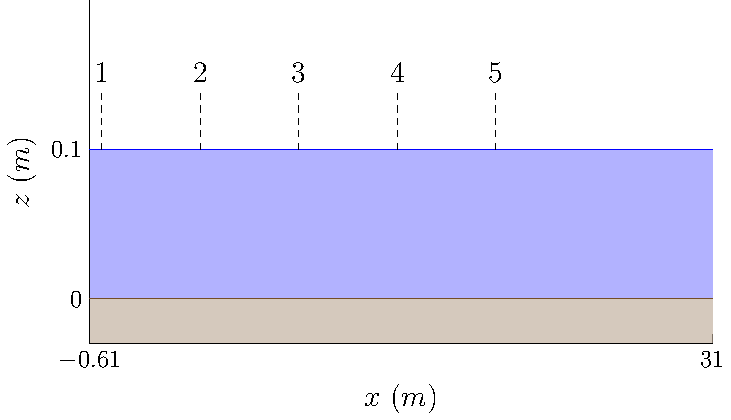
\includegraphics[width=\textwidth]{./chp6/figures/Experiment/Segur/WaveTank.pdf}
	\caption{Diagram showing a longitudinal section of the wave tank for the negative rectangular wave experiments with the water (\squareF{blue}), the bed (\squareF{brown!80!black}) and the WG locations marked.}
	\label{fig:SegurWT}
\end{figure} 

These experiments provide a good benchmark for the capability of the numerical method to accurately model problems with steep gradients in the free surface. These experiments are affected by bed friction, viscosity and the inability of the piston and water to move vertically instantaneously and slip free. The Serre equations do not contain viscosity and bed friction was neglected in this thesis. Additionally, discontinuous initial conditions are used to model the negative rectangular wave. Therefore, we expect that the numerical solutions of the Serre equations may produce many more oscillations in the dispersive wave train than are observed experimentally \cite{Pitt-2018-61}.

\citet{Hammack-Segur-1978-337} report the results for two different initial negative wave amplitudes $0.01m$ and $0.03m$, resulting in the non-linearity parameters $\epsilon = 0.1$ and $\epsilon=0.3$ respectively. Since these non-linearity parameters are relatively small there was no breaking of waves throughout the experiment.

This experiment was modelled numerically using the reflected problem, with the left wall of the wave tank as the axis of symmetry. In the numerical experiments the domain is $[-60m,60m]$ and the experiment is run for $ 50s$ with $g = 9.81m/s^2$. For the spatial resolution we set $\Delta x = 0.01m$ while the CFL condition \eqref{eqn:CFLcond} was satisfied using $\Delta t = 0.5 \Delta x / \sqrt{g \; 0.1}$. The limiting parameter $\theta = 1.2$ was used in the reconstruction \eqref{eqn:slopehGrecon} in $\text{FEVM}_2$ and $\text{FDVM}_2$.

The numerical results of $\text{FDVM}_2$ for these experiments produced by me have been published \cite{Zoppou-etal-2017}. They have been extended here with the inclusion of the conservation error of $h$, $G$ and $uh$ in the numerical simulation of both experiments.

\subsection{Results for the $0.01m$ Negative Rectangular Wave}

Plots comparing the numerical and experimental WG data for the $0.01m$ negative rectangular wave are displayed in Figures \ref{fig:Segur1cmFEVM} and \ref{fig:Segur1cmFDVM} for $\text{FEVM}_2$ and $\text{FDVM}_2$ respectively. We present this data using the same dimensionless scales as reported in the original paper \cite{Hammack-Segur-1978-337}. Tables \ref{tab:ConservationSegurFEVM1cm} and \ref{tab:ConservationSegurFDVM1cm} which display the completely numerically calculated error in conservation $C^*$ are also provided. 
\begin{figure}
	\centering
	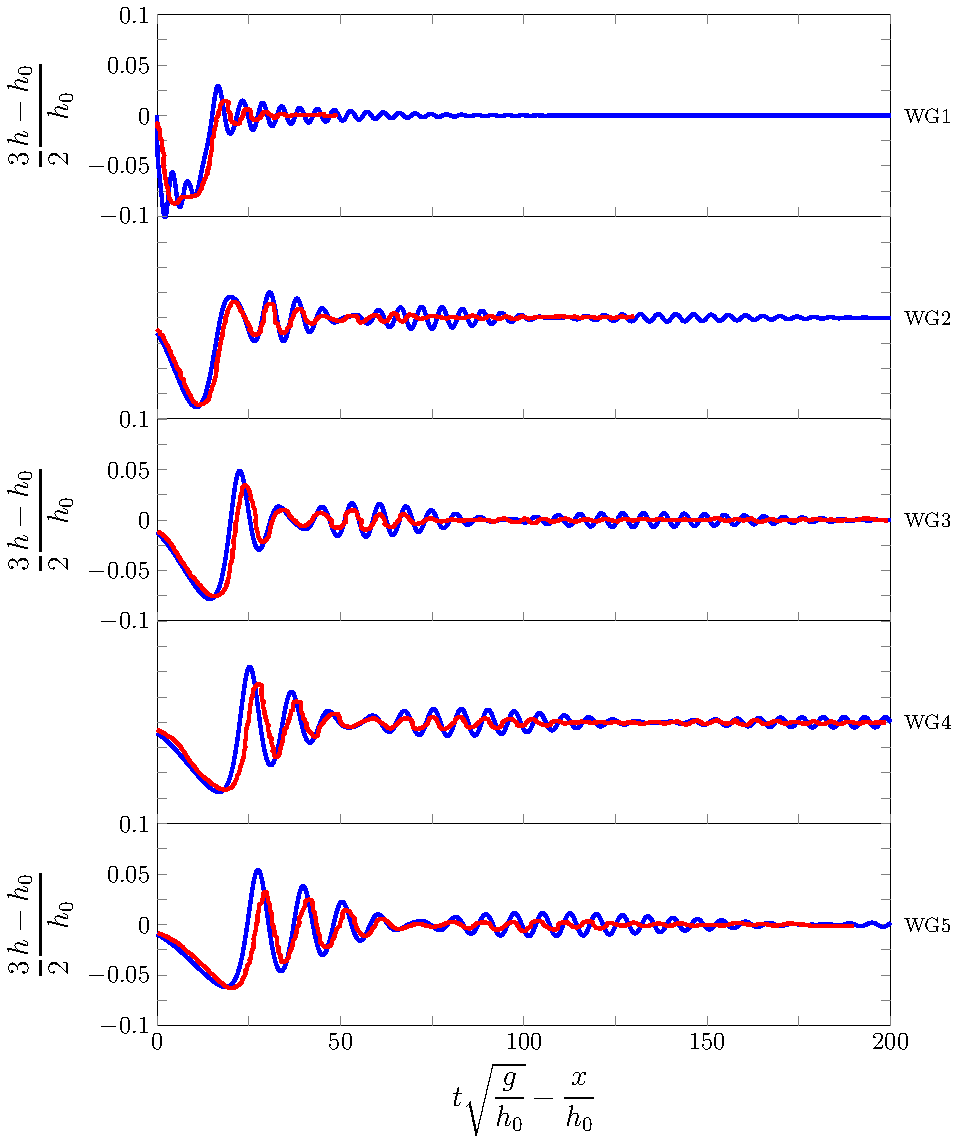
\includegraphics[width=\textwidth]{./chp6/figures/Experiment/Segur/LongWGsFEVM1cm.pdf}
	\caption{Time series of the experimental WG data ({\color{red}\solidrule}) and numerical results ({\color{blue}\solidrule}) of $\text{FEVM}_2$ for the $0.01m$ negative rectangular wave.}
	\label{fig:Segur1cmFEVM}
\end{figure}
\begin{figure}
	\centering
	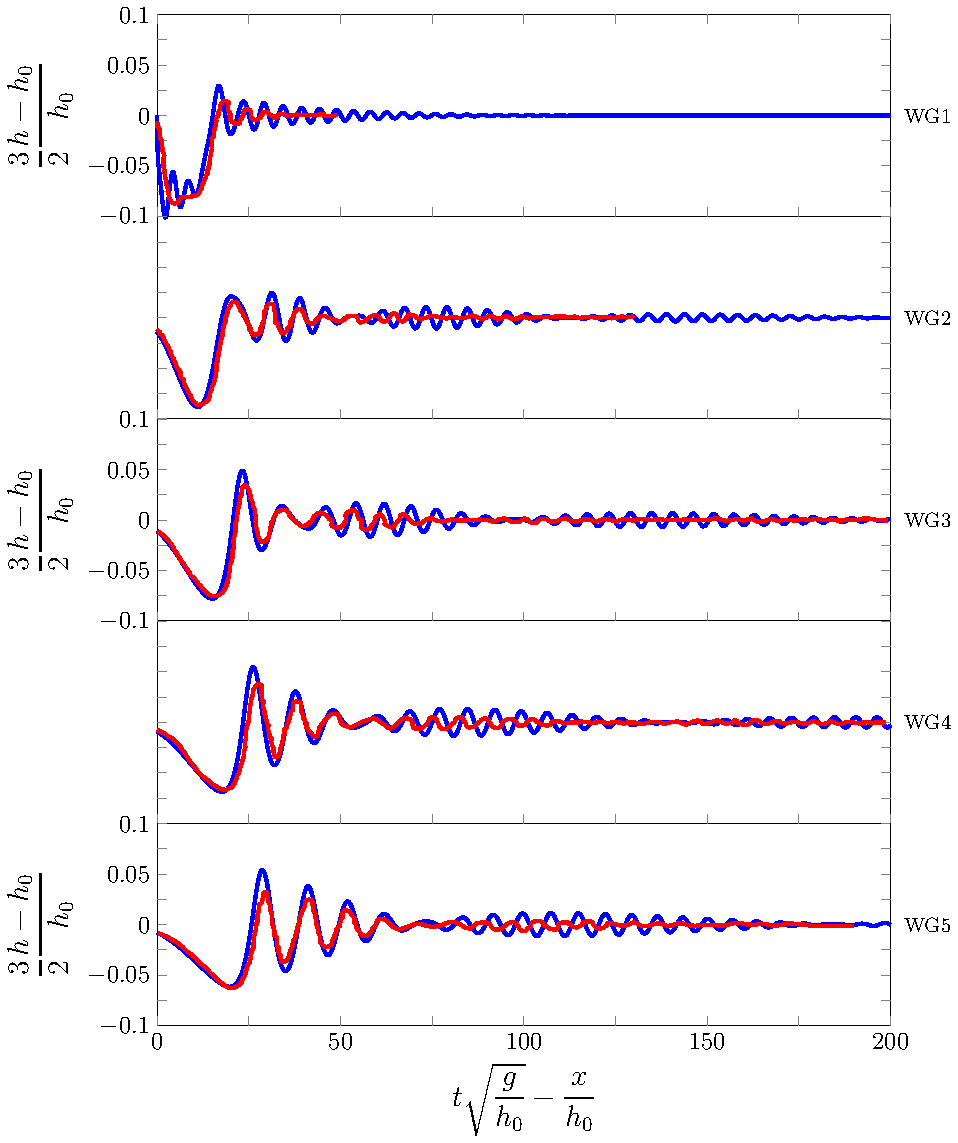
\includegraphics[width=\textwidth]{./chp6/figures/Experiment/Segur/LongWGsFDVM1cm.pdf}
	\caption{Time series of the experimental WG data ({\color{red}\solidrule}) and numerical results ({\color{blue}\solidrule}) of $\text{FDVM}_2$ for the $0.01m$ negative rectangular wave.}
	\label{fig:Segur1cmFDVM}
\end{figure} 

The numerical solutions agree well with the experimental results; particularly for the front of the dispersive wave train. While all the conserved quantities have been conserved well by the methods.

The numerical solutions produce larger and consequently faster waves and generate oscillations in the dispersive wave train which are not present in the experimental data of WG1. Moreover, as expected the methods produce many more oscillations than were observed experimentally. These discrepancies can be attributed to the lack of viscosity and the omission of bed friction for the Serre equations in this thesis \eqref{eqn:FullSerreCon}. Furthermore, it is highly likely the experiment produced some smooth approximation to a discontinuous jump in the water depth with the down-stroke of the piston. Such a smoothing of the initial conditions will significantly attenuate the high frequency waves in the generated dispersive wave train \cite{Pitt-2018-61}. Given these differences the numerical methods do a very good job of replicating the experimental behaviour.

These numerical solutions compare well to those of \citet{Zoppou-etal-2017} for $\text{FDVM}_2$ with $\Delta x = 0.005m$, $\Delta t = 0.2 \Delta t / \sqrt{g 0.1} s$ and $\theta = 1$. Where a higher resolution and a more diffusive value of the limiting parameter were used. These differences had little impact on the WG results. However, the more diffusive value of the limiting parameter smoothed the initial discontinuity which negatively impacted the conservation of $\mathcal{H}$ reported by \citet{Zoppou-etal-2017}.

Both $\text{FEVM}_2$ and $\text{FDVM}_2$ have produced indistinguishable results at this scale and have demonstrated very good conservation of all the quantities see, Tables \ref{tab:ConservationSegurFEVM1cm} and \ref{tab:ConservationSegurFDVM1cm}. Given the extensive examination of several numerical schemes for steep gradient problems \cite{Pitt-2018-61}, this indicates that these solutions are indicative of true solutions of the Serre equations. However, these results do not demonstrate the superiority of one of these methods over the other. 
%
\begin{table}
	\centering
	\begin{tabular}{l  c  c c}
		Quantity& $\mathcal{C}^*\left(\vecn{q}^0\right)$ & $\mathcal{C}^*\left(\vecn{q}^*\right)$ & ${C}^*\left(\vecn{q}^0,\vecn{q}^*\right)$ \B\\
		\hline
		$h$ & $11.9888$ & $11.9888$ & $0$ \T\\
		$uh$ & $0$ & $7.44 \times 10^{-18}$ & $7.44 \times 10^{-18}$\\
		$G$ & $0$ & $1.56\times 10^{-18}$ & $1.56\times 10^{-18}$\\
		$\mathcal{H}$ & $5.8751$ & $5.8751$ & $5.70 \times 10^{-6}$ \B \\
		\hline
	\end{tabular}
	\caption{Initial and final total amounts and the conservation error for all conserved quantities for the numerical solution of $\text{FEVM}_2$ for the $0.01m$ negative rectangular wave.}
	\label{tab:ConservationSegurFEVM1cm}
\end{table} 
%
\begin{table}
	\centering
	\begin{tabular}{l  c  c c}
		Quantity& $\mathcal{C}^*\left(\vecn{q}^0\right)$ & $\mathcal{C}^*\left(\vecn{q}^*\right)$ & ${C}^*\left(\vecn{q}^0,\vecn{q}^*\right)$ \B \\
		\hline
		$h$ & $11.9888$ & $11.9888$ & $0$ \T\\
		$uh$ & $0$ & $-1.19 \times 10^{-17}$ & $-1.19 \times 10^{-17}$\\
		$G$ & $0$ & $-8.05\times 10^{-18}$ & $-8.05\times 10^{-18}$\\
		$\mathcal{H}$ & $5.8751$ & $5.8751$ & $6.27 \times 10^{-6}$ \B\\
		\hline
	\end{tabular}
	\caption{Initial and final total amounts and the conservation error for all conserved quantities for the numerical solution of $\text{FDVM}_2$ for the $0.01m$ negative rectangular wave.}
	\label{tab:ConservationSegurFDVM1cm}
\end{table}  
 

\subsection{Results for the $0.03m$ Negative Rectangular Wave}
The WG data for the numerical and experimental results for the evolution of the $0.03m$ negative rectangular wave are displayed in Figures \ref{fig:Segur3cmFEVM} and \ref{fig:Segur3cmFDVM} for $\text{FEVM}_2$ and $\text{FDVM}_2$ respectively. These results are reported using the same dimensionless scales as in the original paper \cite{Hammack-Segur-1978-337}. The completely numerically calculated conservation error $C^*$ of all the conserved quantities are given in Tables \ref{tab:ConservationSegurFEVM3cm} and \ref{tab:ConservationSegurFDVM3cm} for $\text{FEVM}_2$ and $\text{FDVM}_2$ respectively.
\begin{figure}
	\centering
	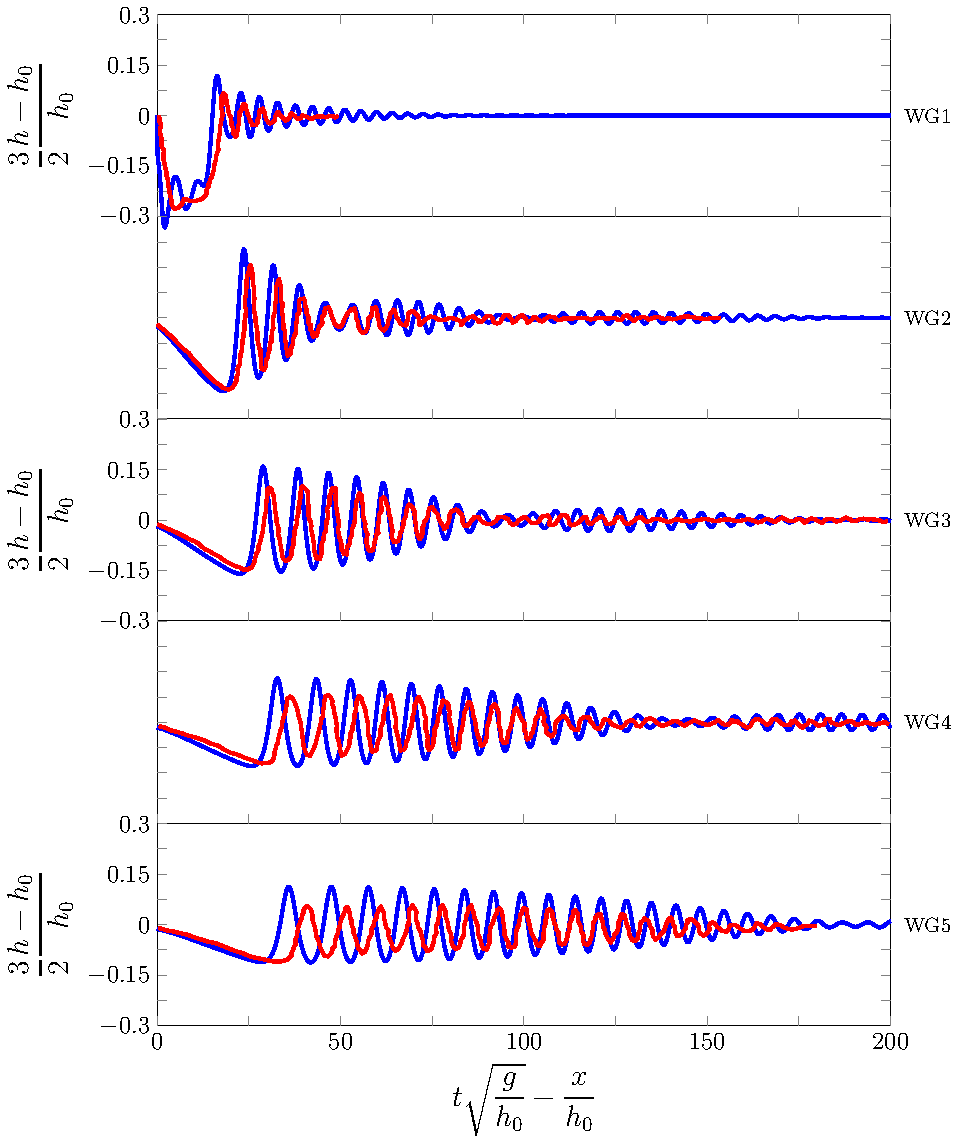
\includegraphics[width=\textwidth]{./chp6/figures/Experiment/Segur/LongWGsFEVM3cm.pdf}
	\caption{Time series of the experimental WG data ({\color{red}\solidrule}) and numerical results ({\color{blue}\solidrule}) of $\text{FEVM}_2$ for the $0.03m$ negative rectangular wave.}
	\label{fig:Segur3cmFEVM}
\end{figure}
\begin{figure}
	\centering
	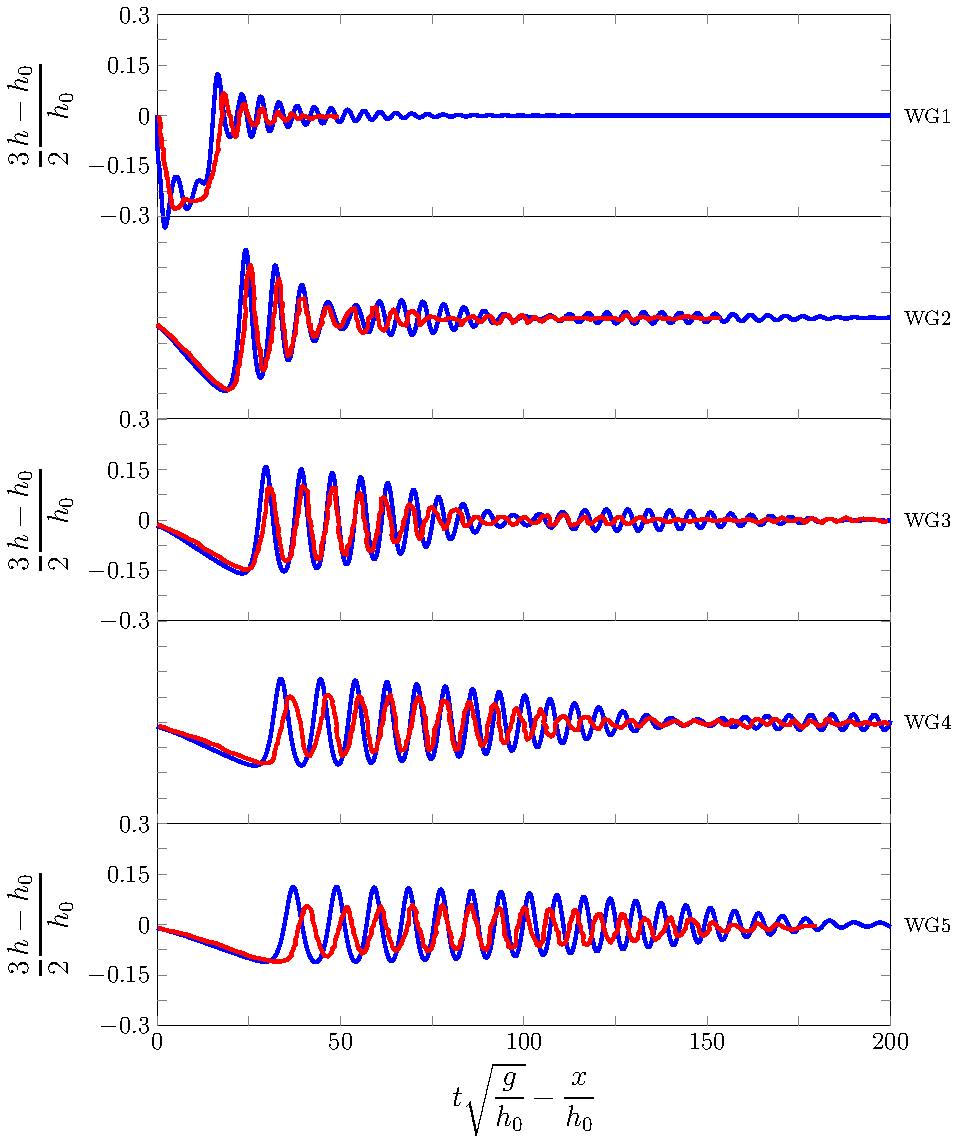
\includegraphics[width=\textwidth]{./chp6/figures/Experiment/Segur/LongWGsFDVM3cm.pdf}
	\caption{Time series of the experimental WG data ({\color{red}\solidrule}) and numerical results ({\color{blue}\solidrule}) of $\text{FDVM}_2$ for the $0.03m$ negative rectangular wave.}
	\label{fig:Segur3cmFDVM}
\end{figure} 

Both methods again reproduce the overall behaviour of this experiment very well. Because the rectangular wave is deeper, this experiment provides a more rigorous test for the numerical methods. However, increasing the depth also strengthens the causes of the discrepancy between the experimental results and the numerical solutions of the Serre equations. Leading to the observed differences for the amplitude and speed of the generated waves.

Since the negative rectangular wave is larger than in the previous example, the numerical methods have a larger error in conservation for all the quantities as compared to the $0.01m$ negative rectangular wave. The exception is the mass which is conserved exactly. For $G$ and momentum these errors are around machine precision and can be disregarded, so that only the conservation of energy is significantly effected. Even with this larger error, all quantities are still well conserved by the numerical methods. 

These results compare well with those by \citet{Zoppou-etal-2017} for $\text{FDVM}_2$ with $\Delta x = 0.005m$, $\Delta t = 0.2 \Delta t / \sqrt{g 0.1} s$ and $\theta = 1$. The WG data of those numerical solutions and the solutions displayed here are indistinguishable. The error in conservation in $\mathcal{H}$ is very similar as well, although in the numerical solutions displayed here the numerical grid is coarser. This is because the limiting parameter $\theta = 1$ diffuses the discontinuous jump, leading to poorer conservation of $\mathcal{H}$ \cite{Pitt-2018-61} than expected given the higher resolution of the grid.

Conserving $\mathcal{H}$ is difficult for numerical methods solving steep gradient problems \cite{Pitt-2018-61}. More so for this simulation where two steep gradients interact with one another over short time spans. Increasing the resolution of the numerical method improves the conservation of $\mathcal{H}$ as demonstrated for the analytic solutions. However, the results for the WG data for higher resolution solutions will be indistinguishable from the results presented here and so the provided solutions are sufficient. 

These experiments have been replicated equally well by the numerical methods. Given the resolution and error in conservation and the extensive study summarised in Chapter \ref{chp:Serreeqns}; these results demonstrate the accuracy of the numerical methods in the presence of steep gradients in the free surface.
%
\begin{table}
	\centering
	\begin{tabular}{l  c  c c}
		Quantity& $\mathcal{C}^*\left(\vecn{q}^0\right)$ & $\mathcal{C}^*\left(\vecn{q}^*\right)$ & ${C}^*\left(\vecn{q}^0,\vecn{q}^*\right)$ \B \\
		\hline 
		$h$ & $11.9644$ & $11.9644$ & $0$ \T\\
		$uh$ & $0$ & $-7.75 \times 10^{-17}$ & $-7.75\times 10^{-17}$\\
		$G$ & $0$ & $-3.33\times 10^{-16}$ & $-3.33\times 10^{-16}$\\
		$\mathcal{H}$ & $5.8560$ & $5.8552$ & $1.24 \times 10^{-4}$  \B \\
		\hline
	\end{tabular}
	\caption{Initial and final total amounts and the conservation error for all conserved quantities for the numerical solution of $\text{FEVM}_2$ for the $0.03m$ negative rectangular wave.}
	\label{tab:ConservationSegurFEVM3cm}
\end{table} 
%
\begin{table}
	\centering
	\begin{tabular}{l  c  c c}
		Quantity& $\mathcal{C}^*\left(\vecn{q}^0\right)$ & $\mathcal{C}^*\left(\vecn{q}^*\right)$ & ${C}^*\left(\vecn{q}^0,\vecn{q}^*\right)$ \B \\
		\hline
		$h$ & $11.9644$ & $11.9644$ & $0$ \T\\
		$uh$ & $0$ & $-9.09 \times 10^{-17}$ & $-9.09 \times 10^{-17}$\\
		$G$ & $0$ & $-1.16\times 10^{-16}$ & $-1.16\times 10^{-16}$\\
		$\mathcal{H}$ & $5.8560$ & $5.8552$ & $1.30 \times 10^{-4}$ \B\\
		\hline
	\end{tabular}
	\caption{Initial and final total amounts and the conservation error for all conserved quantities for the numerical solution of $\text{FDVM}_2$ for the $0.03m$ negative rectangular wave.}
	\label{tab:ConservationSegurFDVM3cm}
\end{table}  

\section{Periodic Waves Over A Submerged Bar}
\label{sec:PeriodicWavessubBar}
%Paper 2 needs a mention []
Beji and Battjes conducted a series of experiments investigating the effect of submerged bars on the propagation of periodic waves \cite{Beji-Battjes-1993-151,Beji-Battjes-1994-1}. The behaviour of these experiments were mainly driven by the dispersion properties of the waves and their interaction with variations in bathymetry. Therefore, these experiments serve as a benchmark for the ability of the numerical schemes to accurately model the interaction of variable bathymetry and dispersive waves. For our purposes we will focus on the monochromatic wave experiments of \citet{Beji-Battjes-1994-1}.

The experiments of \citet{Beji-Battjes-1994-1} were conducted in a wave tank $37.7m$ long, $0.8m$ wide and $0.75m$ high. A diagram of the longitudinal section of the wave tank is given in Figure \ref{fig:BejiWT}. There are seven WG at the following locations; $5.7m$, $10.5m$, $12.5m$, $13.5m$, $14.5m$, $15.7m$ and $17.3m$. Waves are generated from a piston-type wave maker located at $0m$ and travel on the initially still water $0.4m$ deep to the right, over the submerged trapezoidal bar and are absorbed by a sloping beach.
\begin{figure}
	\centering
	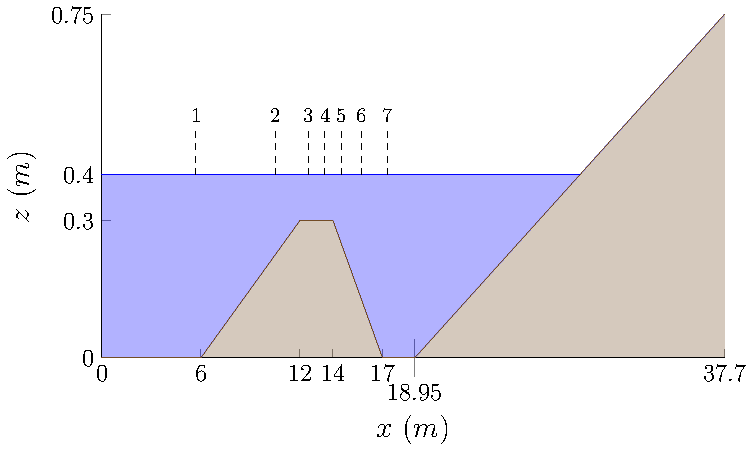
\includegraphics[width=\textwidth]{./chp6/figures/Experiment/Beji/BejiTank.pdf}
	\caption{Diagram showing a longitudinal section of the wave tank for the periodic waves over a submerged bar experiments with the water (\squareF{blue}), the bed (\squareF{brown!80!black}) and the WG locations marked.}
	\label{fig:BejiWT}
\end{figure}

Two monochromatic non-breaking wave experiments were performed. A low frequency one with a wavelength $\lambda \approx 3.69m$ and a period of $T = 2s$, and a high frequency one with $\lambda \approx 2.05m$ and a period of $T = 1.25s$. Both experiments had a wave amplitude of $0.01m$ and so both had the same small non-linearity parameter $\epsilon = 0.01 / 0.4 = 0.025$. 

For the numerical solutions the spatial domain was $\left[5.7m,150m\right]$ with $\Delta x = 0.1 / 2^4 m \approx 0.0063m$ and $\Delta t = Sp / 2^5 s \approx 0.0012s$ where $Sp = 0.039 s$ is the experimental sampling period. These $\Delta x$ and $\Delta t$ values satisfy the CFL condition, \eqref{eqn:CFLcond}. In our numerical experiments only the submerged trapezoidal bar is present, and the sloping beach is replaced with a very long horizontal bed that ensures that we do not observe any effects from the Dirichlet boundary conditions at the downstream boundary.

To simulate the incoming waves at the upstream boundary we used WG1 as our left boundary condition together with linear extrapolation to calculate the other required $h$ values in the left ghost cell. The velocity boundary conditions were calculated from the height values in the same way as \citet{Beji-Battjes-1994-1} using
\begin{equation*}
u(x,t) = \sqrt{g h_0} \; \dfrac{h(x,t) - h_0}{h(x,t)}.
\end{equation*}
Finally the boundary conditions for $G$ were calculated using the boundary values for $h$ and $u$. 

The results of $\text{FDVM}_2$ with the same resolutions and limiting parameter published by \citet{Zoppou-etal-2017} were obtained by me. They have been reproduced here and serve as a comparison for the results of $\text{FEVM}_2$. 

We shall now present our numerical results for the low and high frequency experiments.
%
\subsection{Low Frequency Results}
A comparison of the wave heights $\eta$ of the experimental and numerical results are located in Figures \ref{fig:BejislWG1to4FEVM} and \ref{fig:BejislWG5to7FEVM} for $\text{FEVM}_2$ and Figures \ref{fig:BejislWG1to4FDVM} and \ref{fig:BejislWG5to7FDVM} for $\text{FDVM}_2$. These numerical schemes produce indistinguishable results for all WG and so this benchmark does not help us discriminate between these two methods. 
\begin{figure}
	\centering
	\begin{subfigure}{0.5\textwidth}
		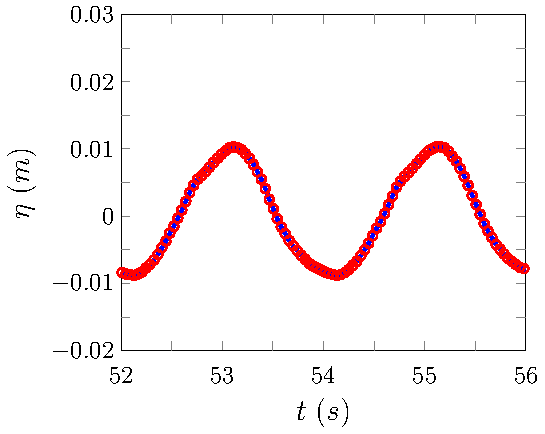
\includegraphics[width=\textwidth]{./chp6/figures/Experiment/Beji/sl/FEVMWG1.pdf}
		\subcaption{WG1}
		\vspace{0.5cm}
	\end{subfigure}%
	\begin{subfigure}{0.5\textwidth}
		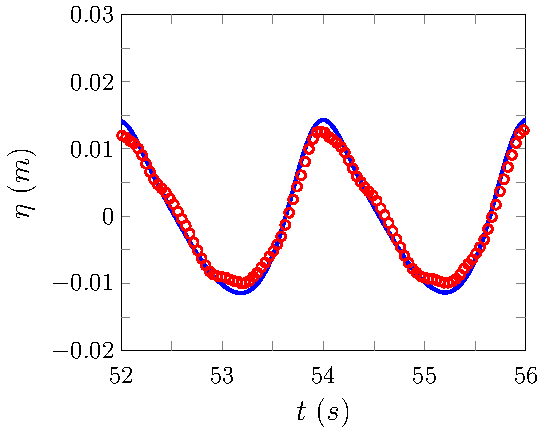
\includegraphics[width=\textwidth]{./chp6/figures/Experiment/Beji/sl/FEVMWG2.pdf}
		\subcaption{WG2}
		\vspace{0.5cm}
	\end{subfigure}
	\begin{subfigure}{0.5\textwidth}
		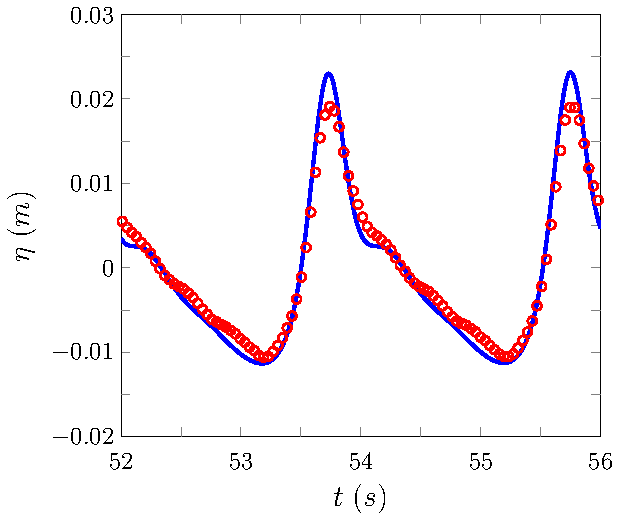
\includegraphics[width=\textwidth]{./chp6/figures/Experiment/Beji/sl/FEVMWG3.pdf}
		\subcaption{WG3}
		\vspace{0.5cm}
	\end{subfigure}%
	\begin{subfigure}{0.5\textwidth}
		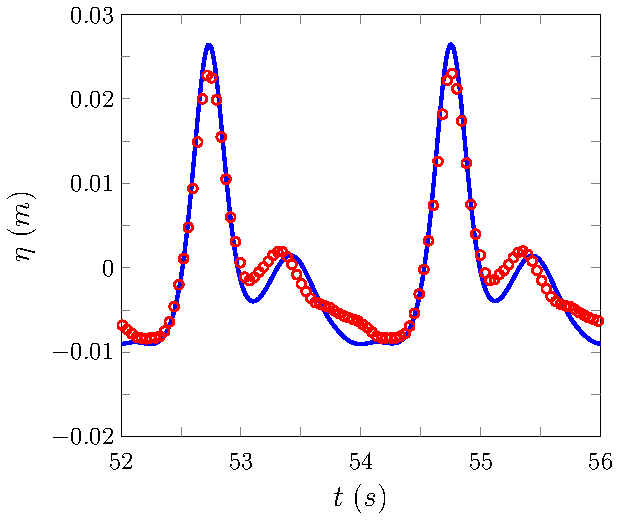
\includegraphics[width=\textwidth]{./chp6/figures/Experiment/Beji/sl/FEVMWG4.pdf}
		\subcaption{WG4}
		\vspace{0.5cm}
	\end{subfigure}
	\caption{Time series of the wave heights $\eta$ of the numerical results of $\text{FEVM}_2$ ({\color{blue}\solidrule}) and the experimental results (\circlet{red}) for WG1 - WG4 for the low frequency experiment.}
	\label{fig:BejislWG1to4FEVM}
\end{figure}
%
\begin{figure}
	\centering
	\begin{subfigure}{0.5\textwidth}
		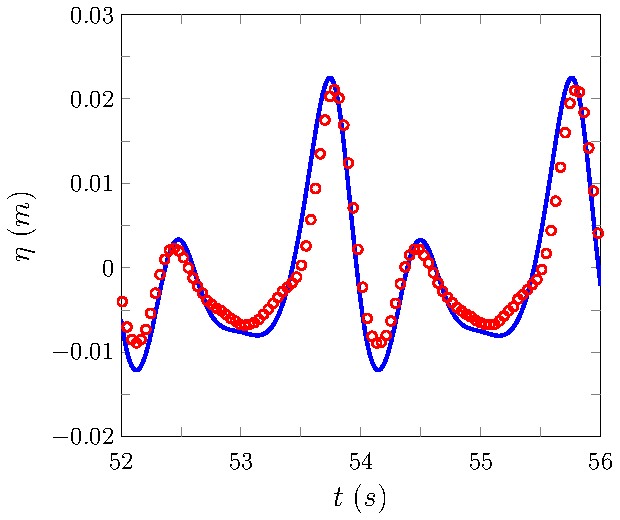
\includegraphics[width=\textwidth]{./chp6/figures/Experiment/Beji/sl/FEVMWG5.pdf}
		\subcaption{WG5}
		\vspace{0.5cm}
	\end{subfigure}%
	\begin{subfigure}{0.5\textwidth}
		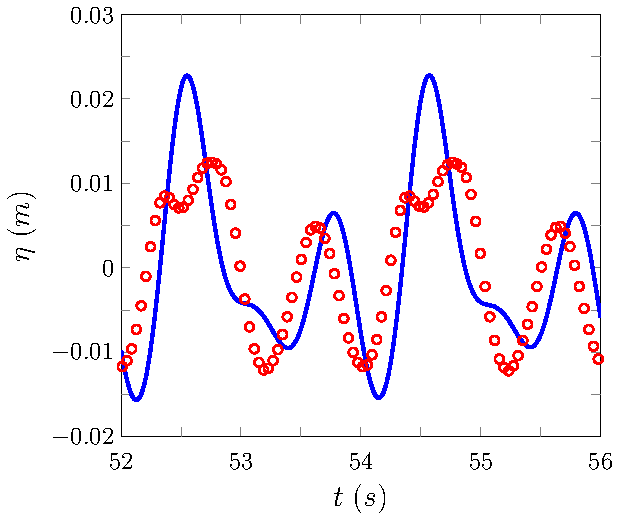
\includegraphics[width=\textwidth]{./chp6/figures/Experiment/Beji/sl/FEVMWG6.pdf}
		\subcaption{WG6}
		\vspace{0.5cm}
	\end{subfigure}
	\begin{subfigure}{0.5\textwidth}
		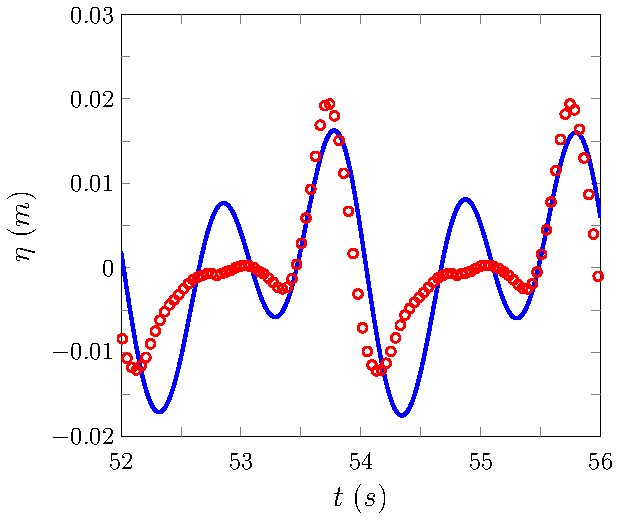
\includegraphics[width=\textwidth]{./chp6/figures/Experiment/Beji/sl/FEVMWG7.pdf}
		\subcaption{WG7}
		\vspace{0.5cm}
	\end{subfigure}
	\caption{Time series of the wave heights $\eta$ of the numerical results of $\text{FEVM}_2$ ({\color{blue}\solidrule}) and the experimental results (\circlet{red}) for WG5 - WG7 for the low frequency experiment.}
	\label{fig:BejislWG5to7FEVM}
\end{figure}
%
\begin{figure}
	\centering
	\begin{subfigure}{0.5\textwidth}
		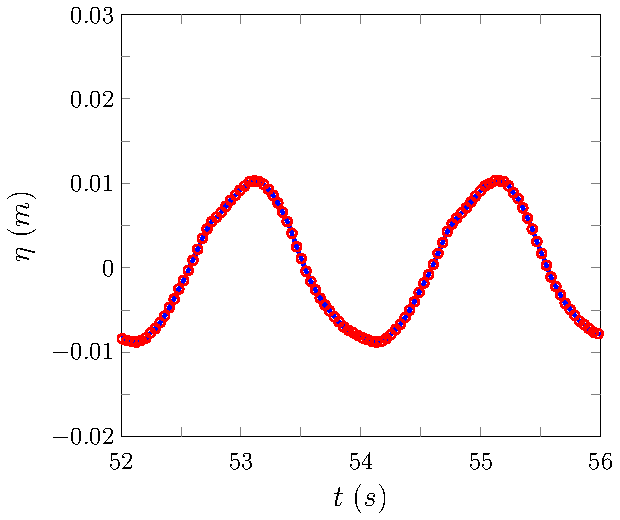
\includegraphics[width=\textwidth]{./chp6/figures/Experiment/Beji/sl/FDVMWG1.pdf}
		\subcaption{WG1}
		\vspace{0.5cm}
	\end{subfigure}%
	\begin{subfigure}{0.5\textwidth}
		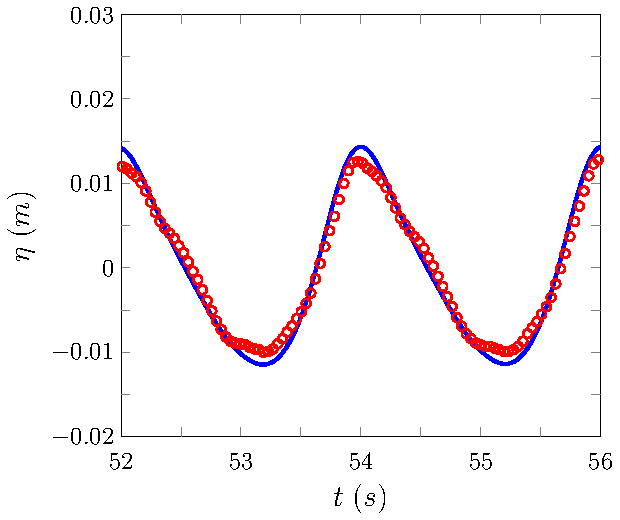
\includegraphics[width=\textwidth]{./chp6/figures/Experiment/Beji/sl/FDVMWG2.pdf}
		\subcaption{WG2}
		\vspace{0.5cm}
	\end{subfigure}
	\begin{subfigure}{0.5\textwidth}
		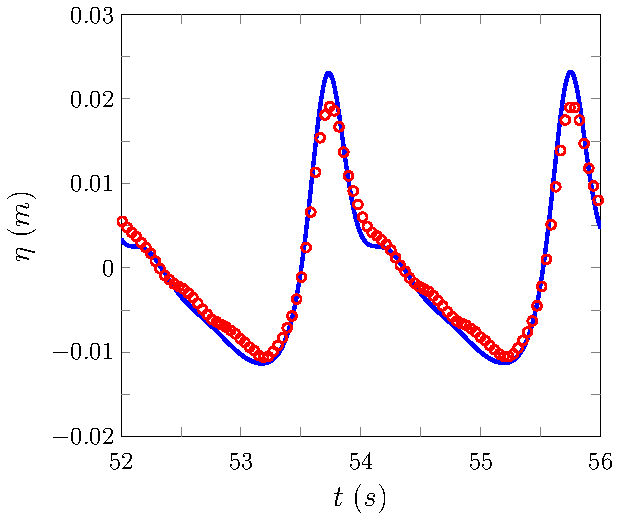
\includegraphics[width=\textwidth]{./chp6/figures/Experiment/Beji/sl/FDVMWG3.pdf}
		\subcaption{WG3}
		\vspace{0.5cm}
	\end{subfigure}%
	\begin{subfigure}{0.5\textwidth}
		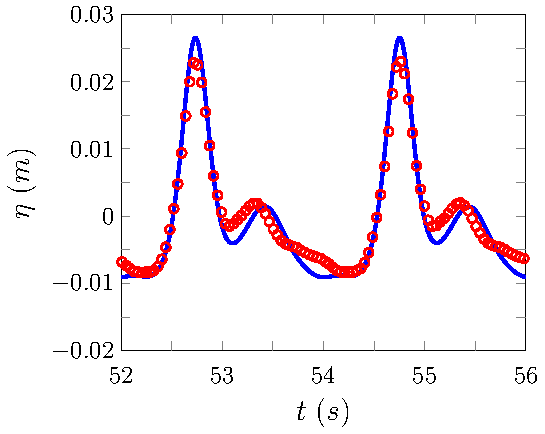
\includegraphics[width=\textwidth]{./chp6/figures/Experiment/Beji/sl/FDVMWG4.pdf}
		\subcaption{WG4}
		\vspace{0.5cm}
	\end{subfigure}
	\caption{Time series of the wave heights $\eta$ of the numerical results of $\text{FDVM}_2$ ({\color{blue}\solidrule}) and the experimental results (\circlet{red}) for WG1 - WG4 for the low frequency experiment.}
	\label{fig:BejislWG1to4FDVM}
\end{figure}
%
\begin{figure}
	\centering
	\begin{subfigure}{0.5\textwidth}
		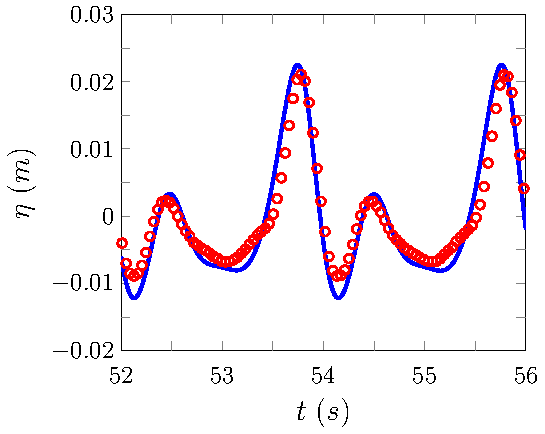
\includegraphics[width=\textwidth]{./chp6/figures/Experiment/Beji/sl/FDVMWG5.pdf}
		\subcaption{WG5}
		\vspace{0.5cm}
	\end{subfigure}%
	\begin{subfigure}{0.5\textwidth}
		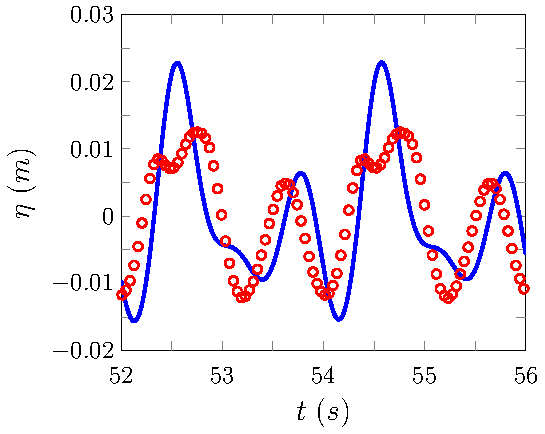
\includegraphics[width=\textwidth]{./chp6/figures/Experiment/Beji/sl/FDVMWG6.pdf}
		\subcaption{WG6}
		\vspace{0.5cm}
	\end{subfigure}
	\begin{subfigure}{0.5\textwidth}
		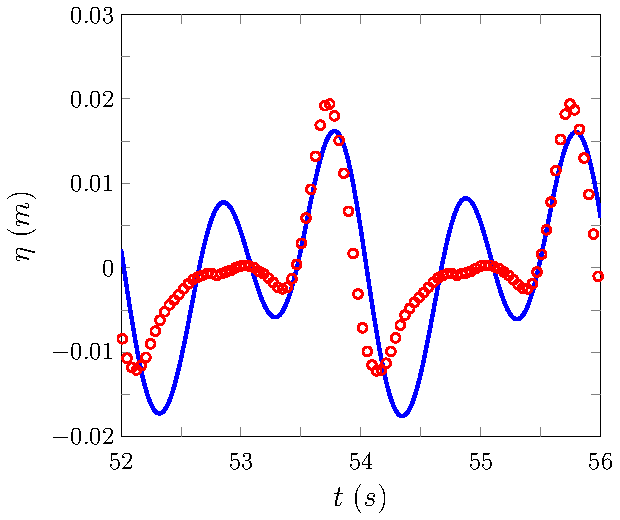
\includegraphics[width=\textwidth]{./chp6/figures/Experiment/Beji/sl/FDVMWG7.pdf}
		\subcaption{WG7}
		\vspace{0.5cm}
	\end{subfigure}
	\caption{Time series of the wave heights $\eta$ of the numerical results of $\text{FDVM}_2$ ({\color{blue}\solidrule}) and the experimental results (\circlet{red}) for WG5 - WG7 for the low frequency experiment.}
	\label{fig:BejislWG5to7FDVM}
\end{figure}

These results demonstrate the ability of these numerical methods to reproduce the experimental results, particularly for WG1 to WG5 where the agreement between experimental and numerical results is best. Results at these gauges validate the numerical schemes for simulating shoaling of dispersive waves as these WG are all located on the windward side of the submerged bar where shoaling occurs in the experiment. 

The numerical results for WG6 and WG7 on the leeward side capture some of the wave behaviour but their agreement with the experiments results is much worse. The inadequacy of the numerical results here appears to be due to the discrepancy between the dispersion properties of the Serre equations and actual water waves \cite{Beji-Battjes-1994-1,Lannes-2013}.

The dispersion terms in the Serre equations are vital to recreating the experimental results for WG2 to WG5, as non-dispersive equations such as the SWWE are not capable of accurately simulating this experiment \cite{Pitt-2017-1725}.

\subsection{High Frequency Results}
The wave heights of the experimental and numerical results are given in Figures \ref{fig:BejishWG1to4FEVM} and \ref{fig:BejishWG5to7FEVM} for $\text{FEVM}_2$. While the results for $\text{FDVM}_2$ are given in Figures \ref{fig:BejishWG1to4FDVM} and \ref{fig:BejishWG5to7FDVM}. As for the low frequency experiment $\text{FEVM}_2$ and $\text{FDVM}_2$ produce indistinguishable results for all WG at this scale and so this benchmark does not discriminate between these two methods. 
%
\begin{figure}
	\centering
	\begin{subfigure}{0.5\textwidth}
		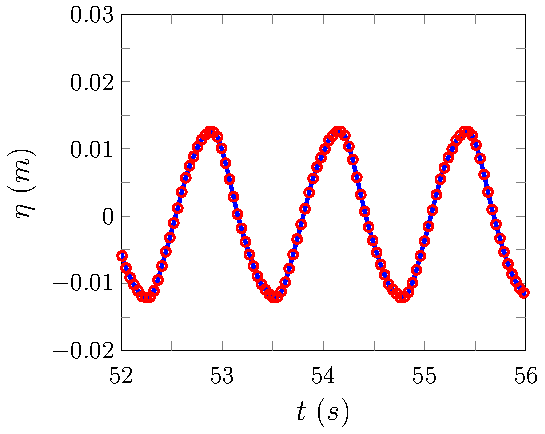
\includegraphics[width=\textwidth]{./chp6/figures/Experiment/Beji/sh/FEVMWG1.pdf}
		\subcaption{WG1}
		\vspace{0.5cm}
	\end{subfigure}%
	\begin{subfigure}{0.5\textwidth}
		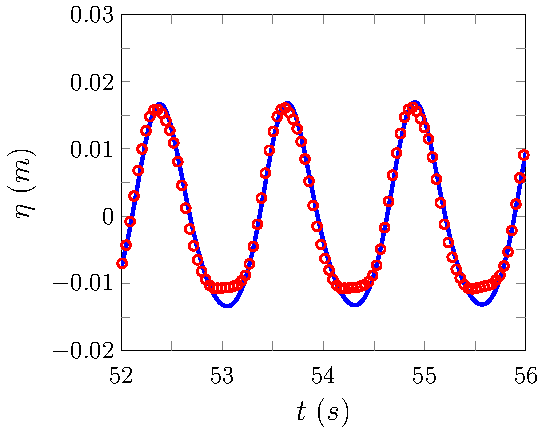
\includegraphics[width=\textwidth]{./chp6/figures/Experiment/Beji/sh/FEVMWG2.pdf}
		\subcaption{WG2}
		\vspace{0.5cm}
	\end{subfigure}
	\begin{subfigure}{0.5\textwidth}
		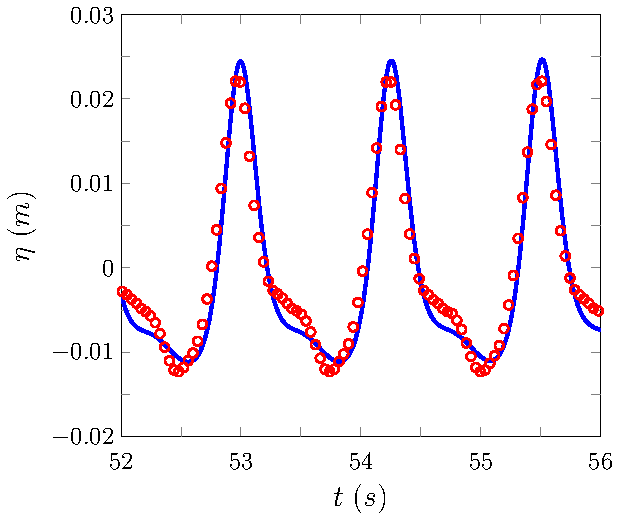
\includegraphics[width=\textwidth]{./chp6/figures/Experiment/Beji/sh/FEVMWG3.pdf}
		\subcaption{WG3}
		\vspace{0.5cm}
	\end{subfigure}%
	\begin{subfigure}{0.5\textwidth}
		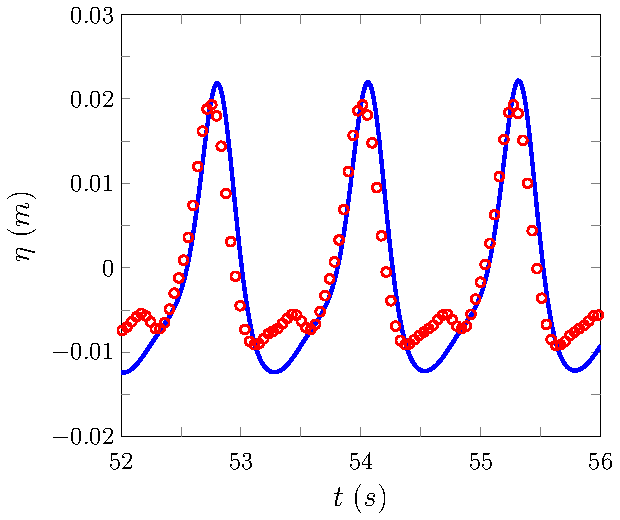
\includegraphics[width=\textwidth]{./chp6/figures/Experiment/Beji/sh/FEVMWG4.pdf}
		\subcaption{WG4}
		\vspace{0.5cm}
	\end{subfigure}
	\caption{Time series of the wave heights $\eta$ of the numerical results of $\text{FEVM}_2$ ({\color{blue}\solidrule}) and the experimental results (\circlet{red}) for WG1 - WG4 for the high frequency experiment.}
	\label{fig:BejishWG1to4FEVM}
\end{figure}
%
\begin{figure}
	\centering
	\begin{subfigure}{0.5\textwidth}
		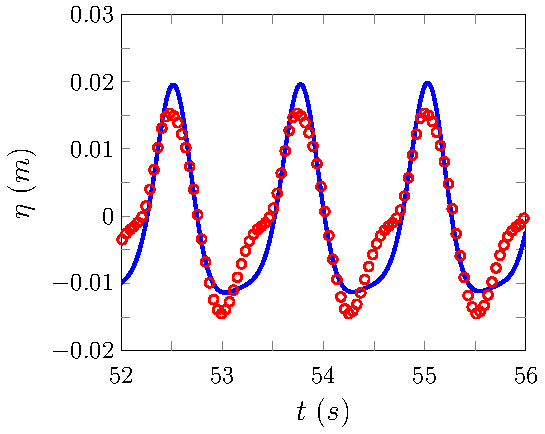
\includegraphics[width=\textwidth]{./chp6/figures/Experiment/Beji/sh/FEVMWG5.pdf}
		\subcaption{WG5}
		\vspace{0.5cm}
	\end{subfigure}%
	\begin{subfigure}{0.5\textwidth}
		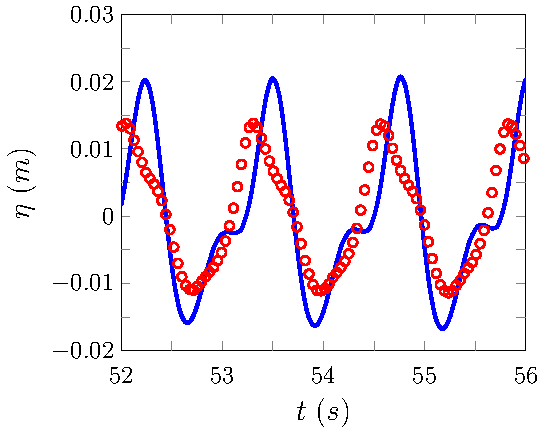
\includegraphics[width=\textwidth]{./chp6/figures/Experiment/Beji/sh/FEVMWG6.pdf}
		\subcaption{WG6}
		\vspace{0.5cm}
	\end{subfigure}
	\begin{subfigure}{0.5\textwidth}
		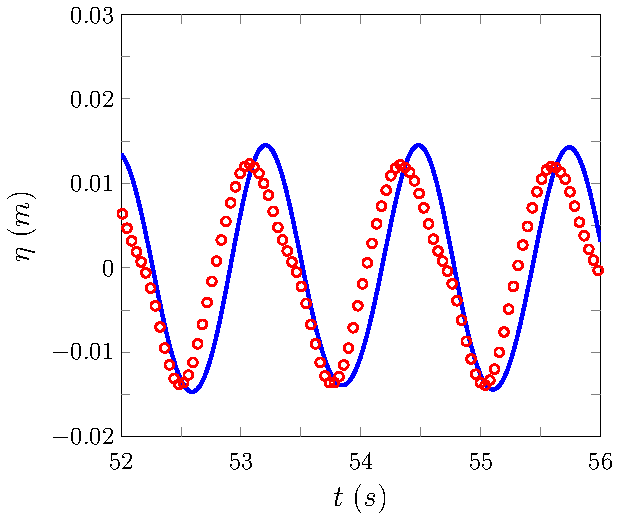
\includegraphics[width=\textwidth]{./chp6/figures/Experiment/Beji/sh/FEVMWG7.pdf}
		\subcaption{WG7}
		\vspace{0.5cm}
	\end{subfigure}
	\caption{Time series of the wave heights $\eta$ of the numerical results of $\text{FEVM}_2$ ({\color{blue}\solidrule}) and the experimental results (\circlet{red}) for WG5 - WG7 for the high frequency experiment.}
	\label{fig:BejishWG5to7FEVM}
\end{figure}
%
\begin{figure}
	\centering
	\begin{subfigure}{0.5\textwidth}
		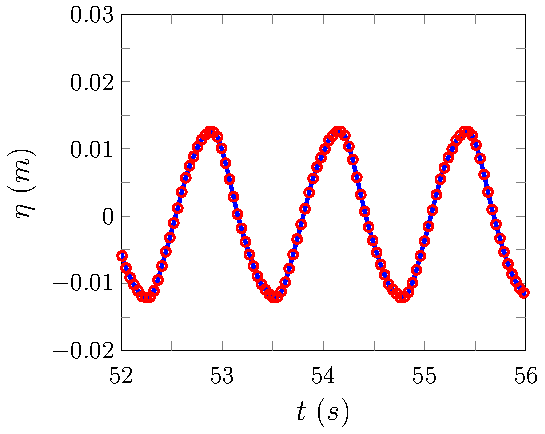
\includegraphics[width=\textwidth]{./chp6/figures/Experiment/Beji/sh/FDVMWG1.pdf}
		\subcaption{WG1}
		\vspace{0.5cm}
	\end{subfigure}%
	\begin{subfigure}{0.5\textwidth}
		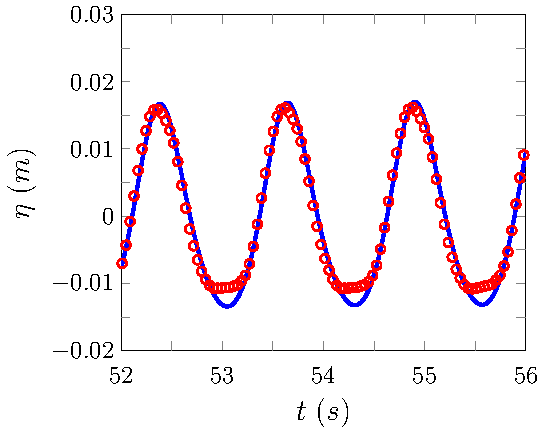
\includegraphics[width=\textwidth]{./chp6/figures/Experiment/Beji/sh/FDVMWG2.pdf}
		\subcaption{WG2}
		\vspace{0.5cm}
	\end{subfigure}
	\begin{subfigure}{0.5\textwidth}
		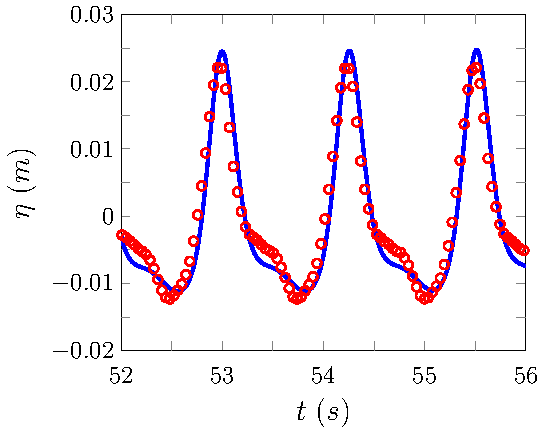
\includegraphics[width=\textwidth]{./chp6/figures/Experiment/Beji/sh/FDVMWG3.pdf}
		\subcaption{WG3}
		\vspace{0.5cm}
	\end{subfigure}%
	\begin{subfigure}{0.5\textwidth}
		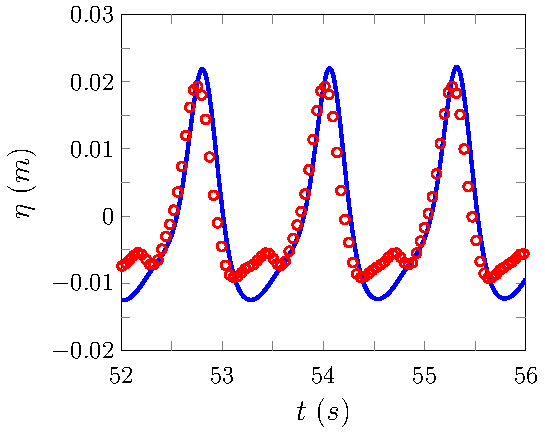
\includegraphics[width=\textwidth]{./chp6/figures/Experiment/Beji/sh/FDVMWG4.pdf}
		\subcaption{WG4}
		\vspace{0.5cm}
	\end{subfigure}
	\caption{Time series of the wave heights $\eta$ of the numerical results of $\text{FDVM}_2$ ({\color{blue}\solidrule}) and the experimental results (\circlet{red}) for WG1 - WG4 for the high frequency experiment.}
	\label{fig:BejishWG1to4FDVM}
\end{figure}
%
\begin{figure}
	\centering
	\begin{subfigure}{0.5\textwidth}
		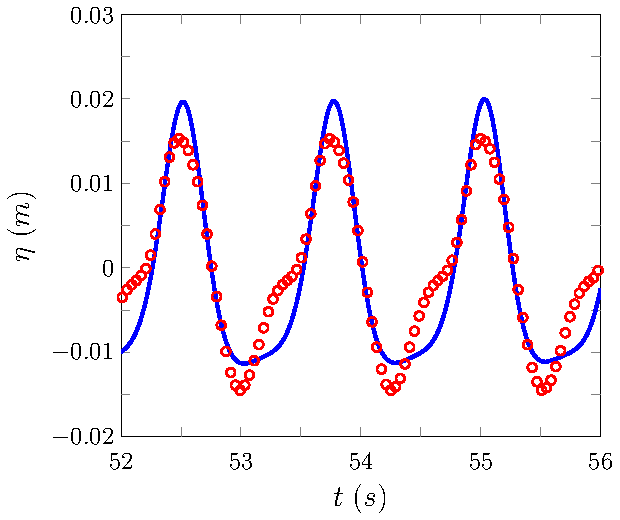
\includegraphics[width=\textwidth]{./chp6/figures/Experiment/Beji/sh/FDVMWG5.pdf}
		\subcaption{WG5}
		\vspace{0.5cm}
	\end{subfigure}%
	\begin{subfigure}{0.5\textwidth}
		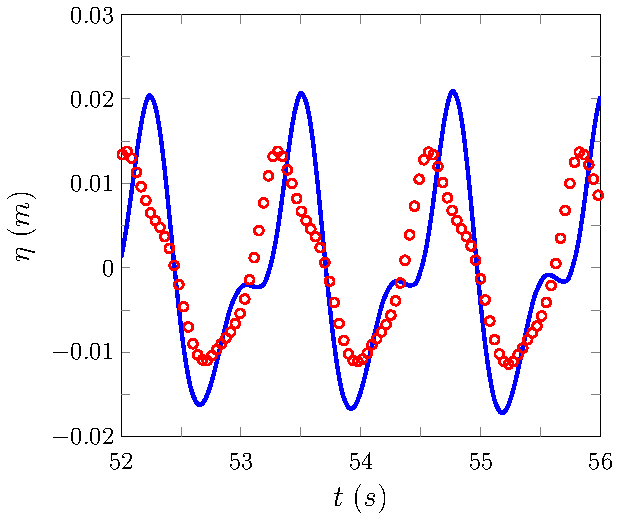
\includegraphics[width=\textwidth]{./chp6/figures/Experiment/Beji/sh/FDVMWG6.pdf}
		\subcaption{WG6}
		\vspace{0.5cm}
	\end{subfigure}
	\begin{subfigure}{0.5\textwidth}
		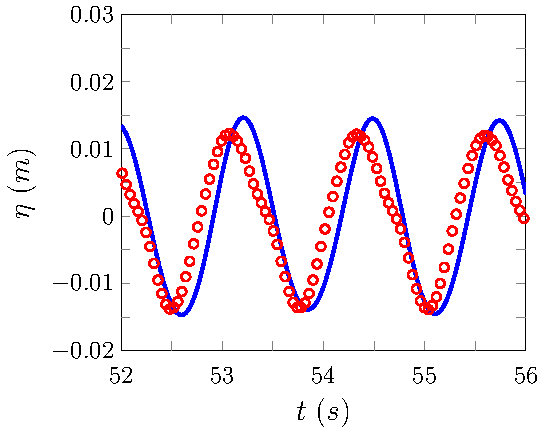
\includegraphics[width=\textwidth]{./chp6/figures/Experiment/Beji/sh/FDVMWG7.pdf}
		\subcaption{WG7}
		\vspace{0.5cm}
	\end{subfigure}
	\caption{Time series of the wave heights $\eta$ of the numerical results of $\text{FDVM}_2$ ({\color{blue}\solidrule}) and the experimental results (\circlet{red}) for WG5 - WG7 for the high frequency experiment.}
	\label{fig:BejishWG5to7FDVM}
\end{figure}

As in the low frequency experiment we observe that the numerical results perform well on the windward side of the slope for WG1 to WG4 but perform poorly for the leeward side of the slope for WG5 to WG7. With the high frequency experiment we see the divergence between the numerical and experimental results earlier than the low frequency experiment, so that now WG5 which is on the leeward side exhibits a significant difference between the numerical and experimental results. As in the low frequency example this is caused by the difference in the dispersion relations of the Serre equations and the linear theory for water waves \cite{Beji-Battjes-1994-1,Lannes-2013}. Because the difference between the dispersion relation of the Serre equations and water waves is largest for higher frequency waves \cite{Barthelemy-2004-315} the earlier divergence between experimental and numerical results is not surprising. 

These numerical results for the $\text{FDVM}_2$ and $\text{FEVM}_2$ agree well with other numerical results for weakly dispersive equations for the simulation of periodic waves over a submerged bar in the literature \cite{Beji-Battjes-1994-1,Lannes-2013,Li-2014-169,Zhang-2013-13}. Therefore, without changing the underlying partial differential equations, our numerical methods perform as well as other numerical schemes in the literature at recreating the experimental results of \citet{Beji-Battjes-1994-1}.

\section{Solitary Wave Over a Fringing Reef}
%Chris wants more nonlinear, shallow water paramtrers there
To study the evolution of waves on fringing reefs a series of experiments were conducted by \citet{Roeber-2010}. These experiments were performed in a wave tank $3.66m$ wide, $83.7m$ long and $4.57m$ high with a removable bed that allowed for the wide range of experiments reported by \citet{Roeber-2010}. We have computationally modelled the experiment with the bathymetry displayed in Figure \ref{fig:RoeberWT}, where a solitary wave is generated from the wave maker at $0m$ and is recorded at the WG located $17.6m$, $28.6m$, $35.9m$, $40.6m$, $44.3m$, $46.1m$, $48.2m$, $50.4m$, $54.4m$, $58.0m$, $61.7m$, $65.4m$, $72.7m$ and $80.0m$ downstream of the wave maker.
\begin{figure}
	\centering
	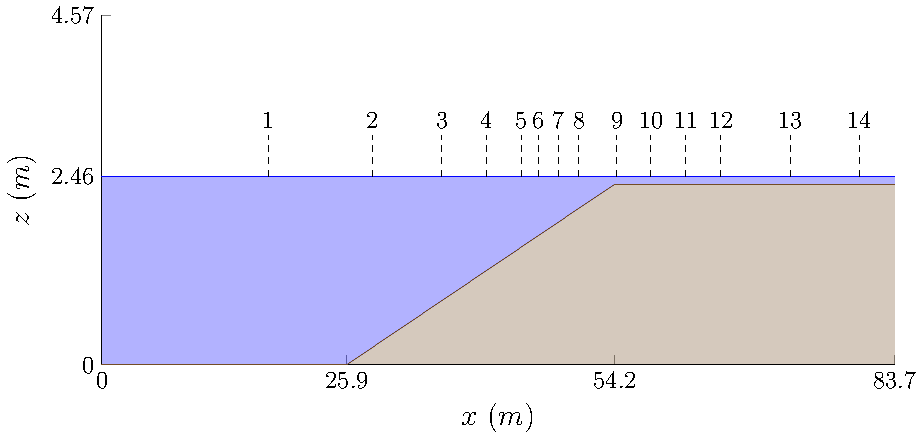
\includegraphics[width=\textwidth]{./chp6/figures/Experiment/Roeber/Trial8/WaveTank.pdf}
	\caption{Diagram showing a longitudinal section of the wave tank for the solitary wave over a fringing reef experiment with the water (\squareF{blue}), the bed (\squareF{brown!80!black}) and the WG locations marked.}
	\label{fig:RoeberWT}
\end{figure}

This experiment investigates the behaviour of a wave with high non-linearity $ \epsilon \approx 1.23/2.46 = 0.5$ as it shoals over a linear bed into a very shallow body of water with a depth of only $0.1m$. Given the high non-linearity of this wave, it is not surprising that as it shoals it becomes a plunging breaker by $t \approx 32s$ with an elliptical air cavity observed at $t \approx 33s$ \cite{Roeber-2010}. As with other depth averaged equations, the Serre equations are only appropriate up to wave-breaking so this experiment is not an entirely appropriate test of the numerical methods, particularly after $t=32s$.

This experiment was numerically modelled on the domain $[17.6m , 400m]$ and was run until $t = 60s$ after which the reflections from the downstream end of the tank become significant in the experiment. The beginning of the domain was chosen so that WG1 could be used as the left boundary conditions. Where the technique for the incoming boundary condition in Section \ref{sec:PeriodicWavessubBar} for the periodic waves over a submerged bar experiment was employed. The spatial resolution was $\Delta x = 0.025m$ and the temporal resolution was $\Delta t = Sp / 8 s = 0.0025$ where $Sp = 0.02s$ was the sampling period of the WG. These spatial and temporal resolutions satisfy the CFL condition \eqref{eqn:CFLcond} for this experiment. The right edge of the domain used Dirichlet boundary conditions, since the domain was large no effects from the downstream boundary were observed throughout the numerical simulation. 

The WG results comparing the numerical and experimental data are displayed in Figures \ref{fig:Roeber8WG1to5FEVM}, \ref{fig:Roeber8WG6to10FEVM} and \ref{fig:Roeber8WG11to14FEVM} for $\text{FEVM}_2$ and \ref{fig:Roeber8WG1to5FDVM} and \ref{fig:Roeber8WG6to9FDVM} for $\text{FDVM}_2$.
\begin{figure}
	\centering
	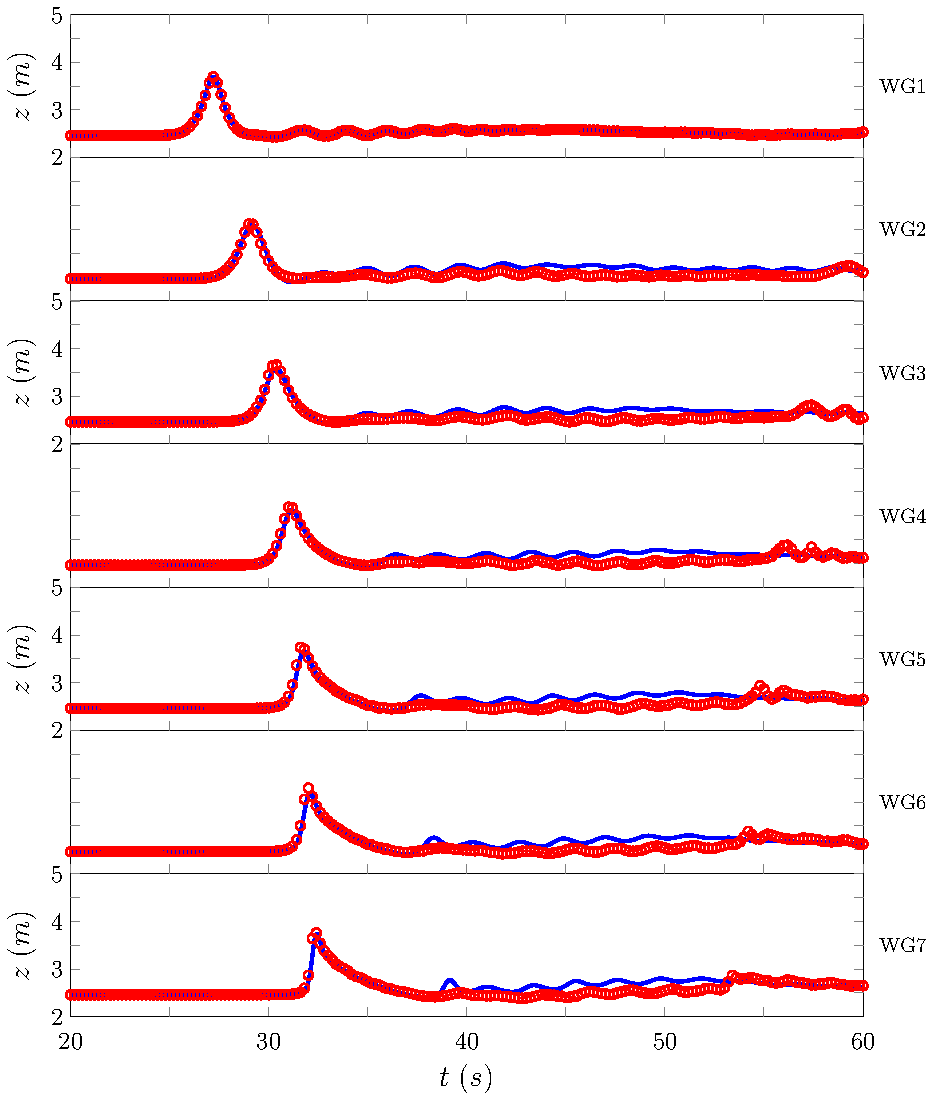
\includegraphics[width=\textwidth]{./chp6/figures/Experiment/Roeber/Trial8/FEVM/LongWGs1.pdf}
	\caption{Time series of the experimental (\circlet{red}) and numerical ({\color{blue}\solidrule}) WG data produced by $\text{FEVM}_2$ for WG1 to WG5.}
	\label{fig:Roeber8WG1to5FEVM}
\end{figure}
\begin{figure}
	\centering
	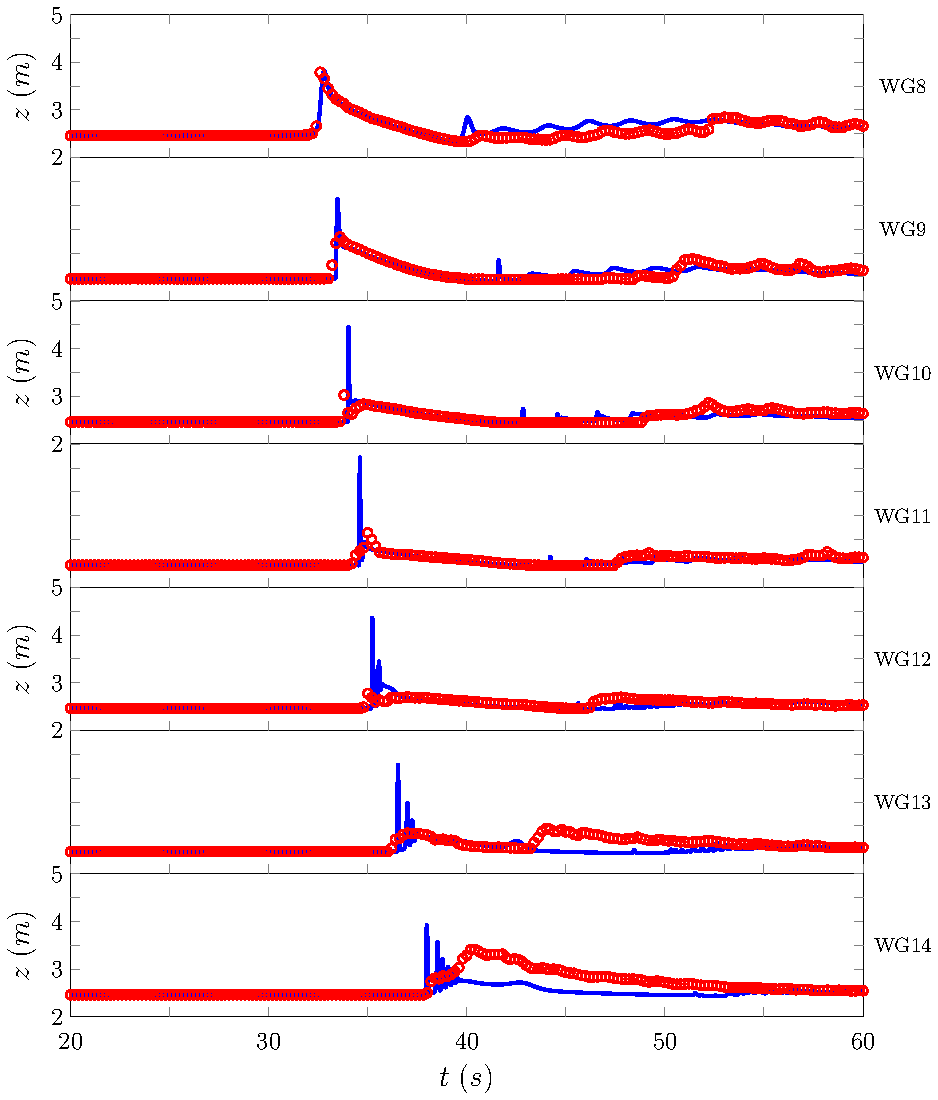
\includegraphics[width=\textwidth]{./chp6/figures/Experiment/Roeber/Trial8/FEVM/LongWGs2.pdf}
	\caption{Time series of the experimental (\circlet{red}) and numerical ({\color{blue}\solidrule}) WG data produced by $\text{FEVM}_2$ for WG6 to WG10.}
	\label{fig:Roeber8WG6to10FEVM}
\end{figure} \begin{figure}
	\centering
	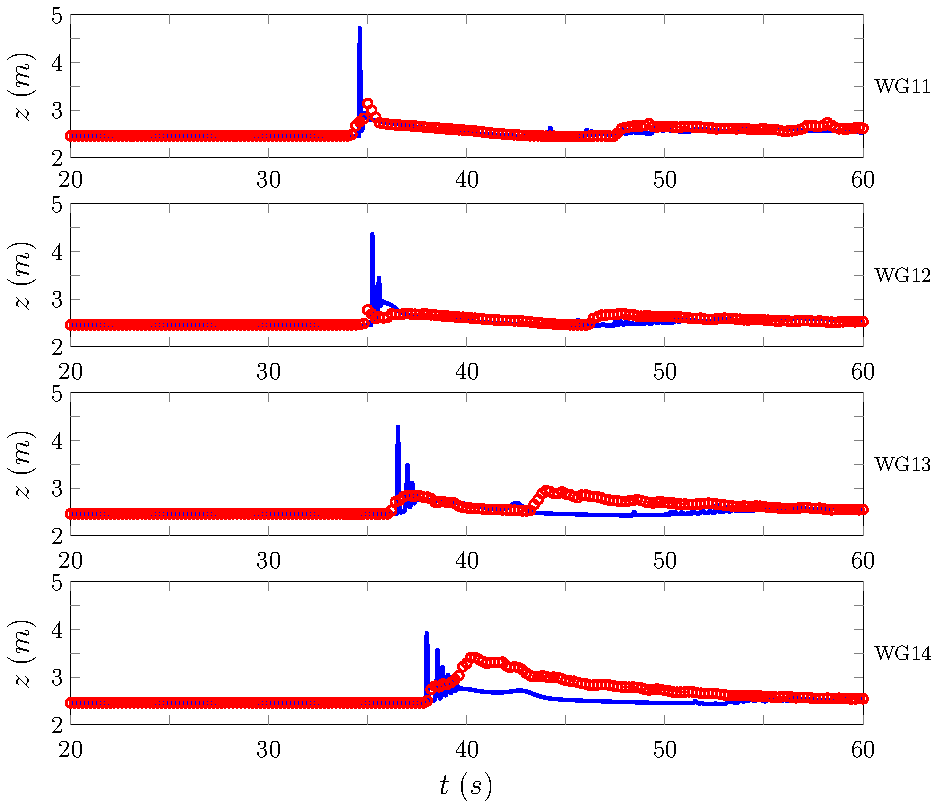
\includegraphics[width=\textwidth]{./chp6/figures/Experiment/Roeber/Trial8/FEVM/LongWGs3.pdf}
	\caption{Time series of the experimental (\circlet{red}) and numerical ({\color{blue}\solidrule}) WG data produced by $\text{FEVM}_2$ for WG11 to WG14.}
	\label{fig:Roeber8WG11to14FEVM}
\end{figure}
\begin{figure}
	\centering
	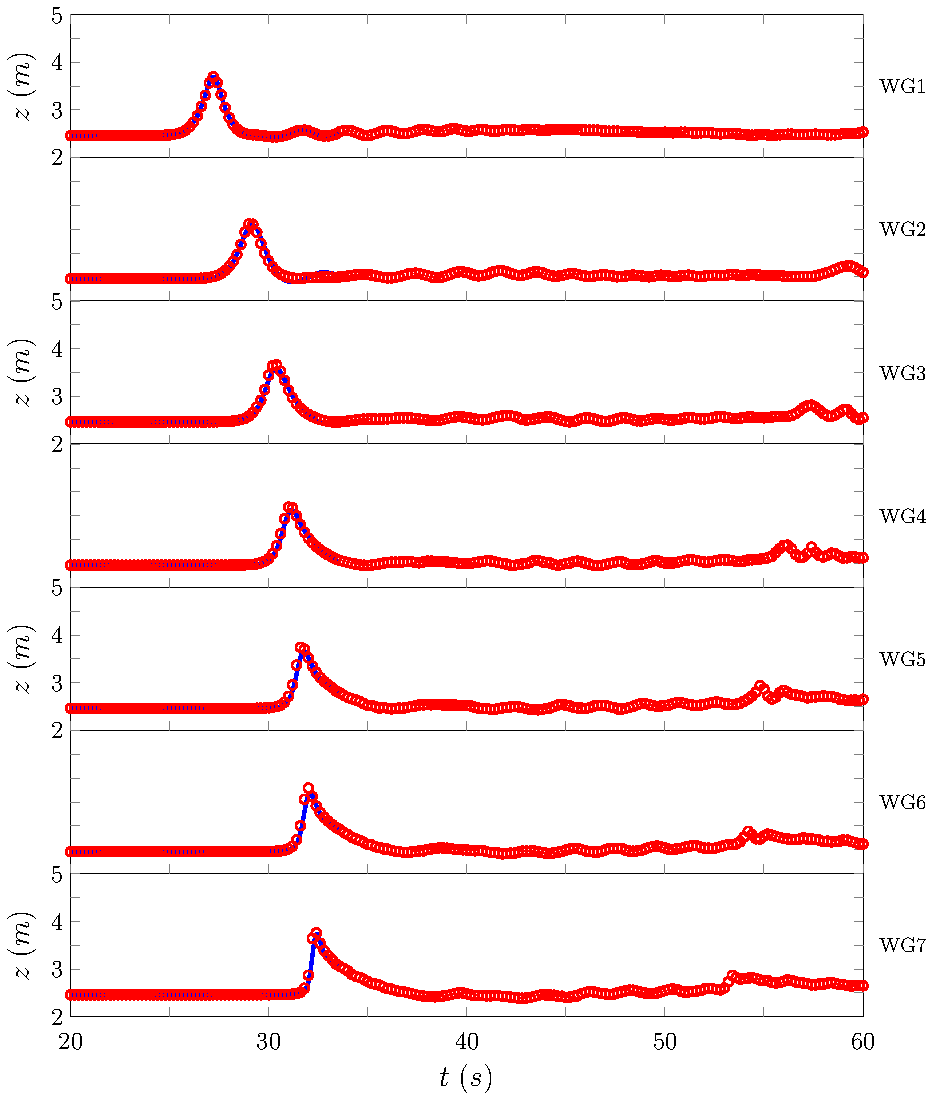
\includegraphics[width=\textwidth]{./chp6/figures/Experiment/Roeber/Trial8/FDVM/LongWGs1.pdf}
	\caption{Time series of the experimental (\circlet{red}) and numerical ({\color{blue}\solidrule}) WG data produced by $\text{FDVM}_2$ for WG1 to WG7.}
	\label{fig:Roeber8WG1to5FDVM}
\end{figure}
\begin{figure}
	\centering
	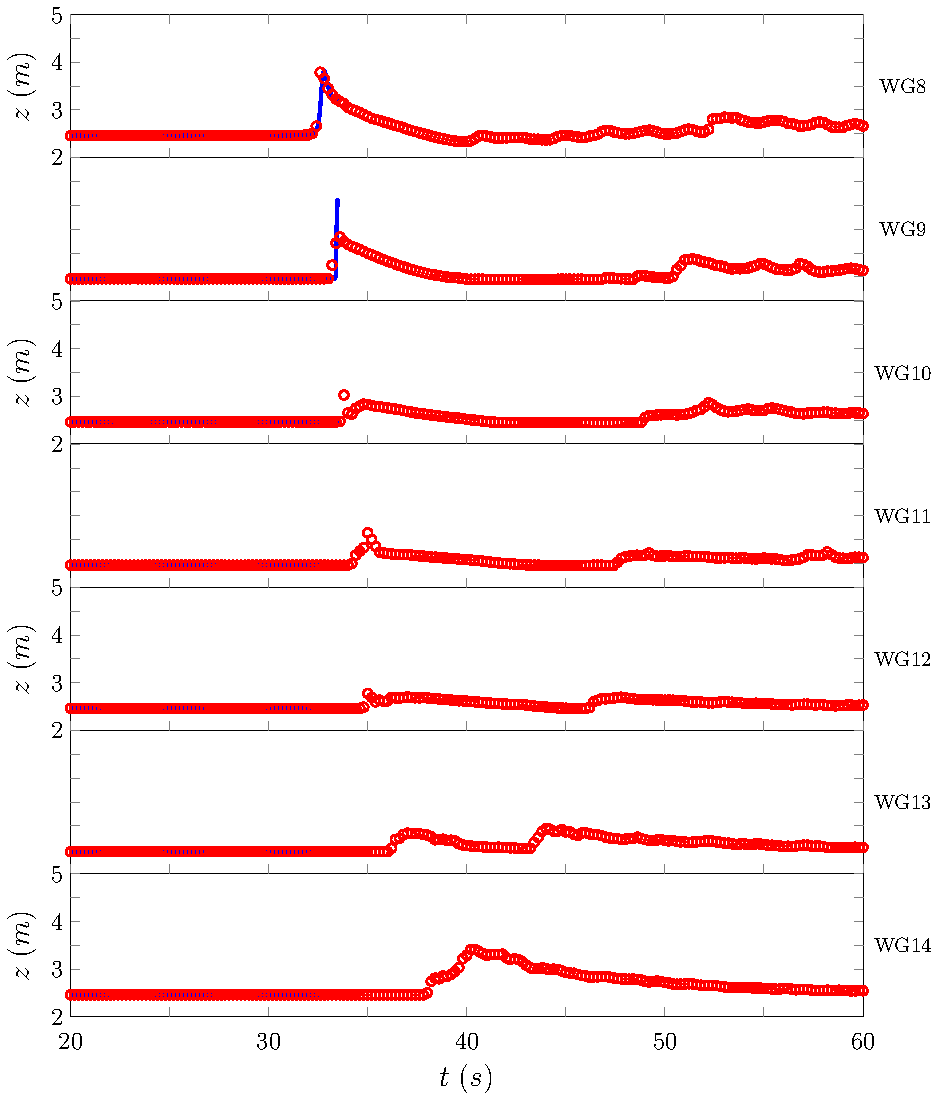
\includegraphics[width=\textwidth]{./chp6/figures/Experiment/Roeber/Trial8/FDVM/LongWGs2.pdf}
	\caption{Time series of the experimental (\circlet{red}) and numerical ({\color{blue}\solidrule}) WG data produced by $\text{FDVM}_2$ for WG6 to WG9.}
	\label{fig:Roeber8WG6to9FDVM}
\end{figure} 

Both methods accurately reproduce the shoaling of the solitary wave, particularly in WG1 through WG8 which record the wave before breaking begins. The behaviour of the trailing waves is not as well replicated, with the numerical solutions overestimating their amplitude and speed as in the previous experiments. The reflected wave can also be observed in the WG and since the numerical simulation did not have reflective boundaries these waves are not replicated in their numerical solutions.

When breaking begins the numerical solutions perform much worse as expected; most notably $\text{FDVM}_2$ becomes unstable and the solution blows up. Because of this the numerical solution of $\text{FDVM}_2$ was only plotted until $t = 34s$. The instability is caused by the appearance of a very steep gradient with a large jump in the water depth compared to the depth of water that surrounds it as the wave breaks. The $\text{FEVM}_2$ method does not suffer from these instability issues, but due to the limitations of the Serre equations does produce a dispersive wave train with amplitudes far exceeding the observed amplitudes in the experiment. 

Given the limitations of the underlying Serre equations the results for $\text{FEVM}_2$ are robust and accurately model the shoaling of the solitary wave. However, these results indicate the need for improvement to the handling of breaking waves to be able to more accurately model some physical situations. 

\section{Run-up Experiment}
To study the run-up of incoming waves on linear beaches a series of experiments were conducted by \citet{Synolakis-1987-523}. These experiments consisted of a number of run-up events for a wide array of breaking and non-breaking waves where snapshots of the entire water surface were taken at certain times. These experiments were all performed on the beach profile depicted in Figure \ref{fig:SynolakisWT}, where all the quantities are non-dimensionalised \cite{Synolakis-1987-523}. To denote that a quantity is non-dimensionalised we use a prime; for example for a generic quantity $q$ its non-dimensionalised version is $q'$. To assess the computational models we recreated one of these experiments, which captured the run-up of a non-breaking solitary wave with a non-linearity parameter of $\epsilon = 0.0185$.
\begin{figure}
	\centering
	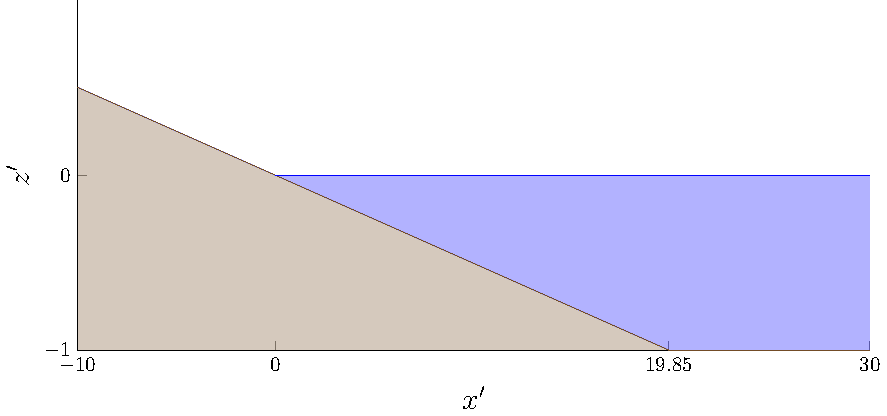
\includegraphics[width=\textwidth]{./chp6/figures/Experiment/Synolakis/WavetankArtifical.pdf}
	\caption{Diagram showing a longitudinal section of the wave tank for the run-up experiment with the water (\squareF{blue}) and the bed (\squareF{brown!80!black}) where the coordinates have been non-dimensionalised \cite{Synolakis-1987-523}.}
	\label{fig:SynolakisWT}
\end{figure}

This experiment allows us to compare the inundation behaviour of our numerical methods with experimental results. For this experiment the effect of dispersion on the run-up behaviour is minimal, and there is good agreement between numerical solutions of the SWWE and this particular experiment \cite{Bollermann-etal-2011-271}. Therefore, the effect of the extra dispersive terms included by the Serre equations on the inundation process is not well tested by this experiment. However, this experiment does demonstrate the robustness of the numerical methods during the wetting and drying of the bed. 

The numerical experiments used the non-dimensionalised quantities reported by \citet{Synolakis-1987-523} to reproduce the experiment. The spatial domain was $x' \in [-30,150]$ with a resolution of $\Delta x = 0.05$ and was run until $t' = 70$ with the CFL condition \eqref{eqn:CFLcond} satisfied by setting $\Delta t = 0.1 \Delta x$. The spatial reconstruction used the input parameter $\theta = 1.2$ and acceleration due to gravity $g= 1$ was chosen to match the non-dimensionalisation.

The non-dimensionalised water surface data is given at the various times in Figure \ref{fig:SynolakisFDVMNoBreak} for $\text{FDVM}_2$ and \ref{fig:SynolakisFEVMNoBreak} for $\text{FEVM}_2$. The error in conservation of $h'$ and $\mathcal{H}'$ as measured by $C^*$ are given in Tables \ref{tab:ConservationSynFEVM} and \ref{tab:ConservationSynFDVM} for $\text{FEVM}_2$ and $\text{FDVM}_2$ respectively. 

\begin{figure}
	\centering
	\begin{subfigure}{0.5\textwidth}
		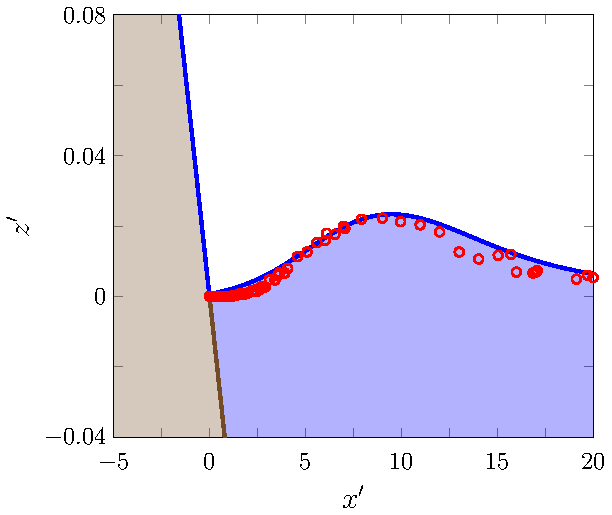
\includegraphics[width=\textwidth]{./chp6/figures/Experiment/Synolakis/H0p0185/FEVM/30s.pdf}
		\subcaption{$t'=30$}
		\vspace{0.5cm}
	\end{subfigure}%
	\begin{subfigure}{0.5\textwidth}
		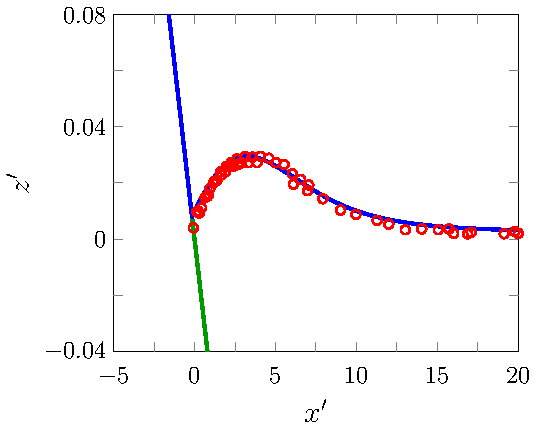
\includegraphics[width=\textwidth]{./chp6/figures/Experiment/Synolakis/H0p0185/FEVM/40s.pdf}
		\subcaption{$t'=40$}
		\vspace{0.5cm}
	\end{subfigure}
	\begin{subfigure}{0.5\textwidth}
		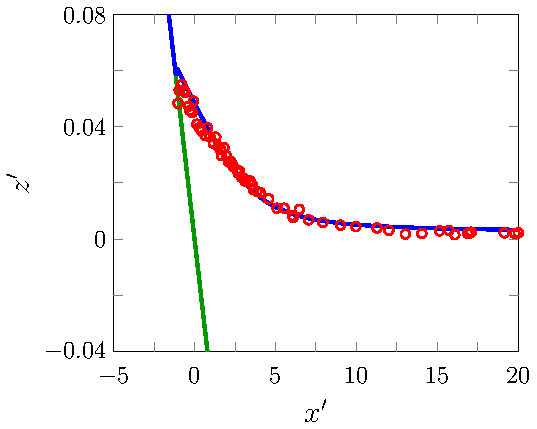
\includegraphics[width=\textwidth]{./chp6/figures/Experiment/Synolakis/H0p0185/FEVM/50s.pdf}
		\subcaption{$t'=50$}
		\vspace{0.5cm}
	\end{subfigure}%
	\begin{subfigure}{0.5\textwidth}
		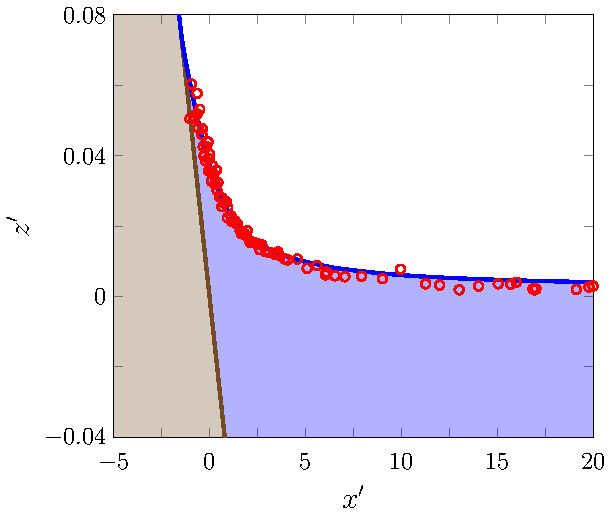
\includegraphics[width=\textwidth]{./chp6/figures/Experiment/Synolakis/H0p0185/FEVM/60s.pdf}
		\subcaption{$t'=60$}
		\vspace{0.5cm}
	\end{subfigure}
	\begin{subfigure}{0.5\textwidth}
		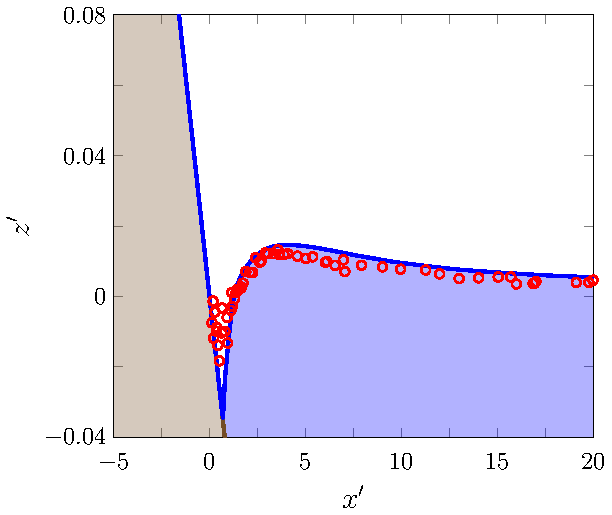
\includegraphics[width=\textwidth]{./chp6/figures/Experiment/Synolakis/H0p0185/FEVM/70s.pdf}
		\subcaption{$t'=70$}
		\vspace{0.5cm}
	\end{subfigure}
	\caption{A comparison of the water surface profiles $w'(x',t')$ for the experiment (\circlet{red}) and the numerical solution (\squareF{blue}) produced by $\text{FEVM}_2$ over the bed (\squareF{brown!60!black}) at various times.}
	\label{fig:SynolakisFEVMNoBreak}
\end{figure}
\begin{figure}
	\centering
	\begin{subfigure}{0.5\textwidth}
		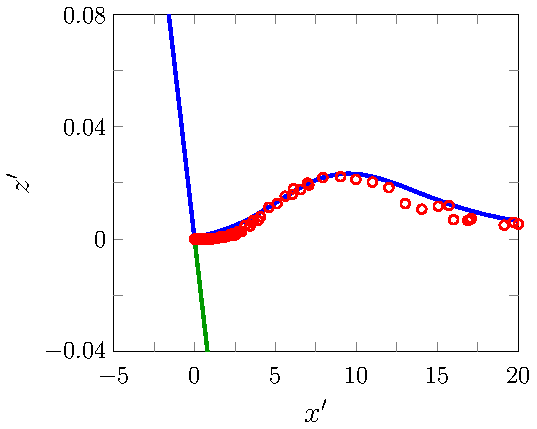
\includegraphics[width=\textwidth]{./chp6/figures/Experiment/Synolakis/H0p0185/FDVM/30s.pdf}
		\subcaption{$t'=30$}
		\vspace{0.5cm}
	\end{subfigure}%
	\begin{subfigure}{0.5\textwidth}
		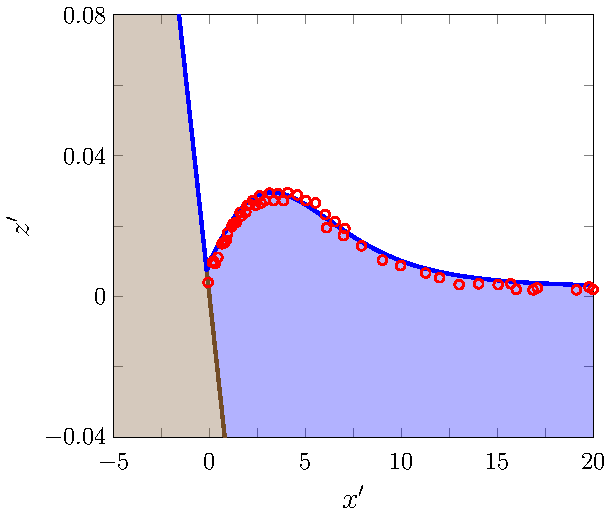
\includegraphics[width=\textwidth]{./chp6/figures/Experiment/Synolakis/H0p0185/FDVM/40s.pdf}
		\subcaption{$t'=40$}
		\vspace{0.5cm}
	\end{subfigure}
	\begin{subfigure}{0.5\textwidth}
		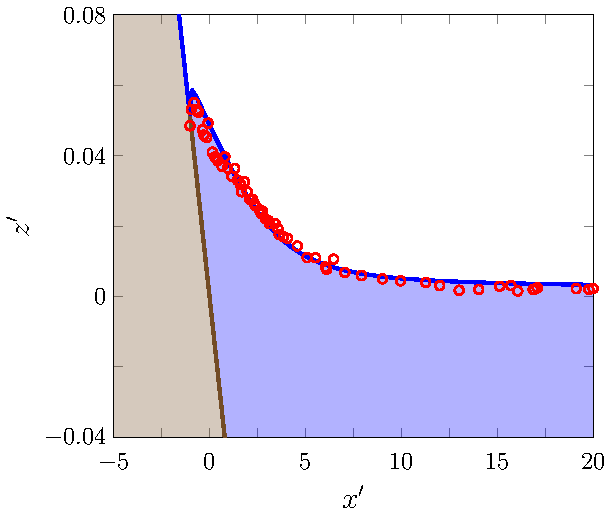
\includegraphics[width=\textwidth]{./chp6/figures/Experiment/Synolakis/H0p0185/FDVM/50s.pdf}
		\subcaption{$t'=50$}
		\vspace{0.5cm}
	\end{subfigure}%
	\begin{subfigure}{0.5\textwidth}
		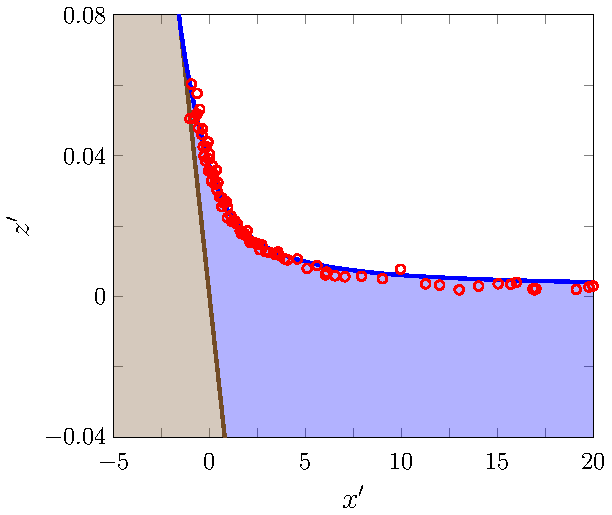
\includegraphics[width=\textwidth]{./chp6/figures/Experiment/Synolakis/H0p0185/FDVM/60s.pdf}
		\subcaption{$t'=60$}
		\vspace{0.5cm}
	\end{subfigure}
	\begin{subfigure}{0.5\textwidth}
		\includegraphics[width=\textwidth]{./chp6/figures/Experiment/Synolakis/H0p0185/FDVM/70s.pdf}
		\subcaption{$t'=70$}
		\vspace{0.5cm}
	\end{subfigure}
	\caption{A comparison of the water surface profiles $w'(x',t')$ for the experiment (\circlet{red}) and the numerical solution (\squareF{blue}) produced by $\text{FDVM}_2$ over the bed (\squareF{brown!60!black}) at various times.}
	\label{fig:SynolakisFDVMNoBreak}
\end{figure}

The results for $\text{FEVM}_2$ and $\text{FDVM}_2$ are indistinguishable, replicating the incoming wave properties and the maximum run-up well. The experimental wave appears to be more skewed towards the shoreline, but this shape difference has all but disappeared as the wave begins to inundate the shore. The only other noticeable difference is that the numerical solutions appear to run-down further than the experimental results. The observed larger run-down is likely caused by the omission of bed friction for the Serre equations in this thesis.

%make sure its understandable
Both $h'$ and $\mathcal{H}'$ are well conserved by the method throughout the run-up and run-down of the wave, particularly $h'$. The total energy $\mathcal{H}'$ of the method is also well conserved, however $\mathcal{H}'$ appears to have slightly increased in the simulation during the run-up process due to the methods handling of the dry bed problem. During this experiment kinetic energy is converted into gravitational potential energy and then back again as the wave is reflected, therefore $u'h'$ and $G'$ will only be conserved in this experiment after the wave has completely reflected from the beach. Full reflection of the wave has not occurred by $t'=70$ and so the conservation results for $uh$ and $G$ were omitted from Tables \ref{tab:ConservationSynFEVM} and \ref{tab:ConservationSynFDVM}.

These numerical solutions demonstrate good agreement with experimental results and display the capability of the method to model the inundation of non-breaking waves.

%Negative energy
\begin{table}
	\centering
	\begin{tabular}{l  c  c c}
		Quantity& $\mathcal{C}^*\left(\vecn{q}^0\right)$ & $\mathcal{C}^*\left(\vecn{q}^*\right)$ & ${C}^*\left(\vecn{q}^0,\vecn{q}^*\right)$  \B\\
		\hline 
		$h'$ & $140.4170$ & $140.4170$ & $7.65\times 10^{-12}$ \T \\
		%$uh$ & $-0.3191$ & $0.3203$ & $0.0040$\\
		%$G$ & $-0.3191$ & $0.3204$ & $0.0043$\\
		$\mathcal{H}'$ & $68.3900$ & $68.3914$ & $2.16 \times 10^{-5}$ \B\\
		\hline
	\end{tabular}
	\caption{Initial and final total amounts and the conservation error for $h'$ and $\mathcal{H}'$ for the numerical solution of $\text{FEVM}_2$ for the run-up experiment.}
	\label{tab:ConservationSynFEVM}
\end{table}
\begin{table}
	\centering
	\begin{tabular}{l  c  c c}
		Quantity& $\mathcal{C}^*\left(\vecn{q}^0\right)$ & $\mathcal{C}^*\left(\vecn{q}^*\right)$ & ${C}^*\left(\vecn{q}^0,\vecn{q}^*\right)$ \B \\
		\hline
		$h'$ & $140.4170$ & $140.4170$ & $1.11\times 10^{-7}$ \T\\
		%$uh$ & $-0.3191$ & $0.3196$ & $0.0017$\\
		%$G$ & $-0.3191$ & $0.3207$ & $0.0050$\\
		$\mathcal{H}'$ & $68.3900$ & $68.3914$ & $2.16 \times 10^{-5}$ \B \\
		\hline
	\end{tabular}
	\caption{Initial and final total amounts and the conservation error for $h'$ and $\mathcal{H}'$ for the numerical solution of $\text{FDVM}_2$ for the run-up experiment.}
	\label{tab:ConservationSynFDVM}
\end{table}

\medskip
In this chapter $\text{FEVM}_2$ and $\text{FDVM}_2$ were validated using experimental data. It was found that for most experiments the solutions of $\text{FEVM}_2$ and $\text{FDVM}_2$ were indistinguishable although $\text{FEVM}_2$ is the preferred method due to its greater robustness. 

